% options:
% thesis=B bachelor's thesis
% thesis=M master's thesis
% czech thesis in Czech language
% english thesis in English language
% hidelinks remove colour boxes around hyperlinks

\documentclass[thesis=B,czech]{FITthesis}[2013/10/20]

\usepackage[utf8]{inputenc} % LaTeX source encoded as UTF-8

\usepackage{graphicx} %graphics files inclusion
% \usepackage{amsmath} %advanced maths
% \usepackage{amssymb} %additional math symbols

\usepackage{dirtree} %directory tree visualisation

\usepackage{float}
\usepackage{wrapfig}
\usepackage{caption}
\usepackage{listings}

\usepackage{courier}

\lstset{basicstyle=\footnotesize\ttfamily,breaklines=true}
\lstset{framextopmargin=50pt}

% % list of acronyms
% \usepackage[acronym,nonumberlist,toc,numberedsection=autolabel]{glossaries}
% \iflanguage{czech}{\renewcommand*{\acronymname}{Seznam pou{\v z}it{\' y}ch zkratek}}{}
% \makeglossaries

\newcommand{\tg}{\mathop{\mathrm{tg}}} %cesky tangens
\newcommand{\cotg}{\mathop{\mathrm{cotg}}} %cesky cotangens

% % % % % % % % % % % % % % % % % % % % % % % % % % % % % % 
% ODTUD DAL VSE ZMENTE
% % % % % % % % % % % % % % % % % % % % % % % % % % % % % % 

\department{Katedra \ldots (Softwarového inženýrství)}
\title{Evidence potravin v OS Android}
\authorGN{Filip} %(křestní) jméno (jména) autora
\authorFN{Kofroň} %příjmení autora
\authorWithDegrees{Filip Kofroň} %jméno autora včetně současných akademických titulů
\supervisor{Ing. Jiří Hunka}
\acknowledgements{Doplňte, máte-li komu a za co děkovat. V~opačném případě úplně odstraňte tento příkaz.}
\abstractCS{Tato bakalářská práce seznamuje čtenáře s globálním problémem plýtvání potravin. Popisuje možné řešení v podobě mobilní aplikace od jeho analýzy, návrhu pro jednoduchost použití a efektivitu, až po implementaci mobilního klienta v prostředí OS Android a serverovou částí využívající svobodný software následovanou testováním. Práce dále hodnotí výsledné řešení a nabízí pohled do jeho budoucnosti s případnými vylepšeními, které přinesla odezva při nasazení aplikace u skutečných uživatelů.}
\abstractEN{Sem doplňte ekvivalent abstraktu Vaší práce v~angličtině.}
\placeForDeclarationOfAuthenticity{V~Praze}
\declarationOfAuthenticityOption{1} %volba Prohlášení
\keywordsCS{Nahraďte seznamem klíčových slov v češtině oddělených čárkou.}
\keywordsEN{Nahraďte seznamem klíčových slov v angličtině oddělených čárkou.}

\begin{document}

% \newacronym{CVUT}{{\v C}VUT}{{\v C}esk{\' e} vysok{\' e} u{\v c}en{\' i} technick{\' e} v Praze}
% \newacronym{FIT}{FIT}{Fakulta informa{\v c}n{\' i}ch technologi{\' i}}

\begin{introduction}

Plýtvání potravin je celosvětový problém, který má přímé následky v plýtvání zdrojů k výrobě potravin, lidského času a sil. Tato činnost je pro mnohé výrobce a zprostředkovatele potravin peněžně výnosná, avšak pro samotnou přírodu včetně fauny a flóry zajisté ne. K chovu zvěře jsou nutné plodiny. Pro růst plodin je třeba prostor, který musíme zabrat na úkor ostatních rostlin a živočichů. Dle British Institution of Mechanical Engineers (IME) byla v roce 2013 odhadnuta skutečnost, že polovinou veškerých potravin na světě je plýtváno~\cite{fakta}.

Během posledních let vzniklo několik projektů, které se různými způsoby snaží tento problém řešit. Jsou to například způsoby domluvy různých lidí o nespotřebovaných potravinách, kdy lidé nabízí co mají navíc a za jiných okolností by vyhodili. Ostatní se mohou domluvit a jídlo si bezplatně či za výhodnou cenu převzít. Tento způsob používa mnoho webovch i mobilních aplikací.

Cílem této práce je vytvořit mobilní aplikaci, která pomůže uživatelům zabránit plýtvání potravin a nabídne jednoduché a rychlé rozhraní, díky kterému bude na uživatele kladena minímální časová náročnost.

V rozvinutých zemích po celém světě je dnes již dostatek potravin a jejich ceny nejsou pro běžné občany likvidační, jak je tomu naopak v některých rozvojových zemích. Přesto se však mnozí lidé snaží ušetřit jejich jmění a nakupovat co nejlevněji. To ovšem například znamená nakupování velkého množství aktuálně cenově výhodných potravin. Takové množství potravin se nemusí vždy podařit včas spotřebovat a lidem tak zůstanou prošlé potraviny, které buď dodatečně spotřebují nebo, pokud si nejsou jistí možnou závadností, potraviny vyhodí do odpadu.

Chytré mobilní telefony vlastní dnes již dostatek lidí na to, aby bylo možné docílit řešení tohoto problému právě skrze mobilní aplikaci. Jelikož je spousta potravin vyhazována do odpadu jen kvůli své opomenuté trvanlivosti, nabízí se řešení v podobě evidence potravin, která uživateli nabídne přehled o trvanlivosti jeho potravin a upozorní ho, pokud nějakým potravinám již trvanlivost skončí, či pokud se tak stane v blízké době.

V této práci popisuji vývoj mobilní aplikace od analýzy až po zhodnocení rozšíření její implementace. Práce využívá znalosti získané během mého studia z předmětů týkajících se algoritmizace, databázových systémů a počítačových sítí.

\end{introduction}

\chapter{Analýza}

Process vývoje musí projít několika následujícími fázemi, při kterých se analyzují všechny aspekty aplikace, které jsou potřeba při návrhu, finalní verifikaci výsledné implementace a jejím testovánim. 

Důraz analýzy je kladen především na potřeby uživatelů, neboť je nutné zaručit minimální nutnou funkcionalitu, která výrazně ovlivní náročnost rozhraní pro pochopení použití i jeho rychlost.

\section{Analýza konkurence}

Tato sekce popisuje aplikace, které více či méně konkurují výsledné aplikaci této práce a snaží se dále popsat jejich vlastnosti. Na konci sekce lze nalézt souhrn, který hodnotí všechny dosavadní řešení a jejich hlavní nedostatky. Informace z této sekce jsou velice důležité pro finální aplikaci. Můžou velice pomoci při hledání cesty k ještě lepšímu řešení než kterými jsou ty konkurenční. Takto lze posbírat důležité poznatky o jejich kladech i záporech, které vyplynou z vlastního otestování (pokud to bude možné) na následujícím seznamu zařízeních, které má autor k dispozici:
\begin{itemize}
  \item{Nexus 7, Android 4.4.2}
  \item{HTC Evo 3D, Android 2.3.4}
  \item{Vodafone 845 (Huawei U8120), Android 2.3.4}
\end{itemize}

V počátku tvorby této práce a implementací aplikace nebylo příliš mnoho konkurenčních aplikací k naleznutí. Jak se však později ukázalo, vzniklo a rozšířilo se během následujících činností několik dalších aplikací, které jen s maálo rozdíly splňují požadavky aplikace výsledkem této práce.

Tato část byla zprvu velice krátka, neboť jediné bližší aplikace neposkytovali vhodné srovnání ani zisk vhodných informací. V závěru jsem však usoudil, že některé tyto aplikace zaslouží zanalyzování a poskytnou tak čtenáři jistý nadhled nad daným tématem i v průběhu následujícího čtení. Dalším důvodem jejich zmiňky je autorovo zmýlení v jejich existenci v počátku, jelikož aplikace byly nedávno uvedené a nebylo dostatek vodítek k jejich naleznutí.

\subsection{Best before}

Aplikace Best Before je zdarma dostupná jak pro zařízení s iOS, tak pro zařízení s OS Android. Na první pohled je aplikace totožná na obou platformách. Při bližším zkoumání verze pro OS Android však bylo zjištěno, že aplikace využívá čisté prvky OS Android v částech jako jsou dialogy a některé běžné komponenty. Toto vytváří silný kontrast v rozhraní, který nemusí být pro uživatele OS Android příjemný přesto, že aplikace je jinak po stránce stylu více než na dobré úrovni.

Samotná funkcionalita aplikace je omezena a čistě přizpůsobena svému účelu. Aplikace disponuje seznamem potravin seřazeným v pořadí, v jakém jednotlivým potravinám vypřší spotřební lhůta. Přidání potraviny do aplikace lze tlačítkem v horním pravém rohu, které při stisku zobrazí jendoduchý formulář, ve kterém lze nastavit obrázek potraviny, název, místo uložení a z dialogu vybrat datum spotřeby.Nelze však zadat již existující potravinu a pokud uživatel zadává více potravin, může takto ztrávit poměrně dlouhou dobu.

Z vlastního testování však byly zjištěny zásadní nedostatky v ošetření různách chyb a stabilitě. Na žádném z použitých zařízení aplikace nebylo možné přidat obrázek potraviny, a při ukládání potraviny došlo při každém k pokusu k pádu, potravina se ve 4 z 5ti pokusů přidala, v jednom došlo ke kompletnímu smazání všech ostatních potravin. Aplikace byla tuďíž nepoužitelná. Z hodnocení na Google Play Store ~\cite{play_store} vyplývá, že někteřým uživatelům aplikace funguje bez problému, jiní naopak hlásí stejné problémy. Celkové hodnocení aplikace na Play Store se v rozsahu 1 až 5 umísťilo na hodnotě 3.9. Vzhledem k použitelnosti je tato hodnota spíše překvapivá.

Ve výsledku lze z této aplikace převzít zejména pozitivní přístup uživatelů k hezky nastylovanému rozhraní, které se zdá být jediným důvodem nadprůměrného hodnocení. Ačkoliv je toto pouze autorův názor, pro ověření by však bylo třeba širšího testování mezi různými uživateli, které ale je příliš časově náročné.

\subsection{Food Safe}

Další aplikací určenou pro Android OS je Food Safe ????, která se objevila na Play Store teprve nedávno, v době psaní tohoto textu přibližne 20 dní. Aplikace představuje přímou konkurenci aplikaci této práce. Informace o této aplikaci byly získány pouze z Play Store z toho důvodu, že nebylo možné nainstalovat aplikaci na žádné ze zařízení, které byly k dispozici při jejím testování v této práci. 

Aplikace není dostupná zadarmo. Je třeba ji zakoupit za částku, která v době psaní tohoto textu činí 20,40 Kč.

U této aplikace lze zaznamenávat potraviny pomocí jména a datumu spotřeby. Aplikace zdá se nabízí i možnost skenování čárových kódů, z hodnocení Play Store je ale zřejmé, že aplikace získává informace o potravinách od uživatelů a zaznamenává je do externí databáze. První uživatelé tedy budou nuceni zadávat ručně detaily všech jednotlivých potravin.

\subsection{Love Food Hate Waste}

Stejně jako aplikace Best Before je tato ve verzích pro iOS i Android OS. Rozhraní aplikace je témeř identické v obou verzích, používá styl a prvky obvyklé pouze pro iOS. Vzhled dává velmi dobrý dojem 
o aplikaci.

Nabízená funkcionalita zahrnuje:
\begin{itemize}
  \item{Recepty}
  \item{Množstevní plán}
  \item{Jídelníček}
  \item{Kuchyň - inventář potravin}
  \item{Nákupní lístek}
\end{itemize}

Z popisu aplikace není dostatek informací o jejich skutečné použitelnosti, z hodnocení uživatelů je ale patrné, že aplikace má mnoho nedostatků, kterými jsou nejčastěji omezení počtu kategorií jídel, zbytečně zobrazené kategorie způsobující nepřehlednost a vysoká nestabilita. Všechny tyto nedostaky vedli uživatele Play Store k celkovému hodnocení 2.5, tedy průměrnou hodnotu.

\subsection{Souhrn analýzy konkurence}

Ze všech výše uvedených aplikací je nejvíce podobná aplikaci této práce aplikace Food Safe. Nabízí možnosti, které usnadňují evidenci potravin, nenutí uživatele zadávat zbytečné informace a sbírá již zadaná data uživateli, aby je mohli použít i ostatní uživatelé. Přesto, že tato aplikace je velice podobná, aplikace této práce má snahu přinést ještě jednodušší způsob zadávání potravin, jejich společné sdílení a pokusit se disponovat více informacemi o potravinách, které do aplikace ještě žádný uživatel nezadal a umožnit takto jednodušší a především rychlejší zadání nové potraviny.

Nejzajímavější nápad aplikace Food Safe je bezesporu možnost načíst čárový kód. Autor si takto troufá tvrdit nejen proto, že informace o čárových kódech jsou dostupné volně na internetu, jak bude dále popsáno, ale také proto, že naprostá většina potravin, které lze koupit v běžných řetezcích, obsahují tyto čárové kódy, které jsou pro ně unikátní.

\section{Cílová skupina uživatelů}

Nepředpokládá se, že by se tato aplikace používala široce například v restauračních a jiných zařízeních disponujících závodními kuchyněmi, kterými prochází mnoho potravin a mobilní telefon pro tuto skupinu uživatelů nebude příliš pohodlný. Přesto však může aplikace stačit nějakému malému podniku, pokud si chce vést jednoduchou evidenci, jen aby předešel plýtvání, které by pro menší kapitál mohl znamenat veliký problém.

Autor však shledal nutnost aplikaci umožnit používat jakémukoliv členu rodiny či domácnosti. Je to zejména proto, aby mohl kdokoliv z rodiny použít rodinný účet a nově zakoupenou potravinu nebo právě spotřebovanou okamžitě přidat do aplikace, respektive odstranit. Nejen pro tento účel, ale i pro výše zmíněné sdílení informací o potravinách bude nutné, aby aplikace disponovala externím úložištěm dat.

Pro širší skupinu použití je vhodné u potravin evidovat i jejich jeden nebo více obrázků, které mohou vhodným způsobem odlišit jednotlivé potraviny i například pro lidi, kteří mají problém přečíst název potraviny, jejíž obrázek však rozpoznají jednodušeji. Autor nepředpokládá, že by tyto cílové skupiny potraviny přímo zadávali, a proto není nutné řešit problém zadání datumu spotřeby i pro tyto uživatele.

\clearpage

\section{Analýza požadavků}

Jako základ dalšího postupu aplikace je seznam jejích požadavků. Je třeba shrnout několik základních znalostí okolo problému, kterému se tato aplikace snaží nalézt řešení.

Prvním aspektem aplikace jako řešení je její rozšíření. Aby aplikace dosáhla k většině uživatelů a stala se tak efektivni, je zapotřebí zvolit takovou platformu, kterou používa nejvíce lidí. Z různých internetových zdrojů lze nalézt, že nejrozšířenější platforma na mobilních telefonech. Protože u žádného z těchto zdrojů nebylo možné zajistit autentičnost, byla k této práci vypracován krátký dotazník, na který odpovědělo 31 lidí. Cílem tohoto dotazníku bylo nalézt zajímavé informace, které pomůžou při výběru cílové platformy, a další informace pomáhající při volbě funkcionality. Výsledek rozšíření platforem mezi dotázanými lze nalézt na obrázku ~\ref{fig:SurveyOS}.

\begin{figure}[H]
  \centering
  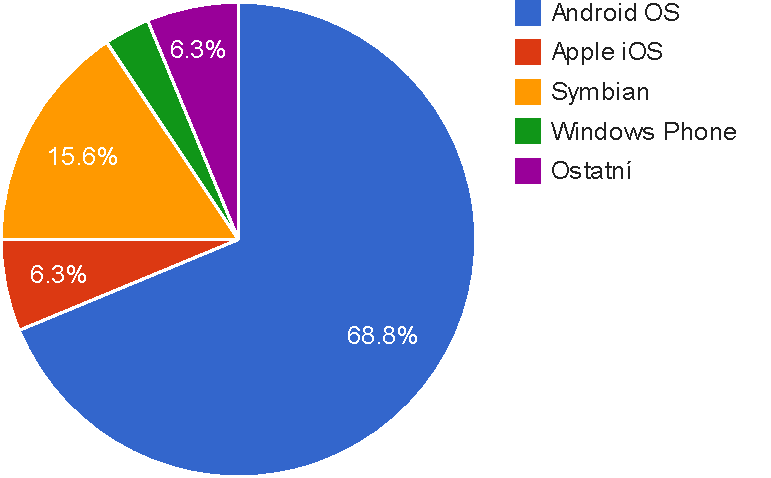
\includegraphics[scale=0.8]{charts/survey_os}
  \caption{Rozšíření mobilních platforem}
  \label{fig:SurveyOS}
\end{figure}

Výběr cílové platformy je tedy jistý. Čtenář může jistě dohledat další průzkumy rozšíření platforem, které jsou více či méně rozdílné, avšak všechny poukazují na fakt, že OS Android je nejrozšířenější. Tato práce si dává za cíl poskytnout řešení pro tuto platformu. Protože budoucnost této aplikace může přinést rozšíření i na více platforem, je nutné zajistit, aby společené úložiště dat aplikace bylo možné použít i pro jinou platformu. Toto zajistí multiplatformní protokol.

Vzhledem k tomu, že většina potravin disponuje čárovým kódem a k tomuto kódu můžou být dohledány informace o zboží, které identifikuje, lze aplikaci vybavit čtečkou čárových kódu, která usnadní manuální zadávání názvu či tohoto kódu. Aby tato informace nebyla jen tak nadhozena, byla do dotazníku přidána další sekce. Na obrázku ~\ref{fig:SurveyScan} lze pozorovat poměr mezi dotázanými, kteří by využili možnosti zadávat jídlo pomocí čtečky a těmi, kteří by toho nevyužili.

\begin{figure}[H]
  \centering
  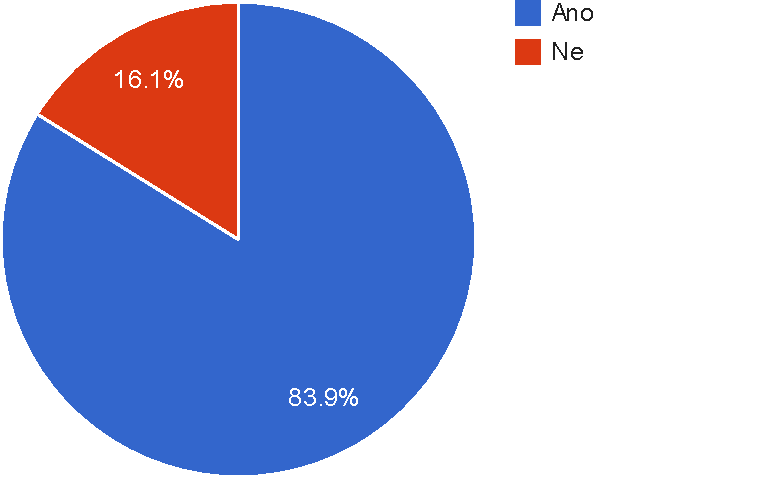
\includegraphics[scale=0.8]{charts/survey_scan}
  \caption{Žádanost zadávání potravin pomocí čtečky čárového kódu}
  \label{fig:SurveyScan}
\end{figure}

Funkční požadavky této aplikace, které plynou z daného problému a výše uvedených výsledků dotazníku jsou:

\begin{itemize}
  \item přidávání nových potravin
  \item sdílení známých potravin
  \item specifikace běžné doby spotřeby potraviny
  \item zaznamenání fotografie potraviny
  \item zaznamenávání potravin do inventáře
  \item odebírání potravin z intentáře
  \item zaznamenání data spotřeby
  \item hledání potraviny pomocí čárového kódu nebo názvu
  \item čtení čárového kódu pomocí kamery mobilního telefonu
  \item upozornění na jídlo, jehož spotřební doba se ocitla v krátkém intervalu mezi koncem, či jehož spotřební doba již uplynula
  \item nastavení intervalu pro upozornění o spotřebě, který je rozdílem doby spotřeby potraviny a aktuálního data
  \item získávání informací o neznámých potravinách z otevřené databáze čárových kódů
\end{itemize}

Android OS se na cílových zařízeních nachází v různých verzích. Některé jsou příliš staré na to, aby je bylo nutné podporovat, jiné jsou naopak ještě stále rozšířené. Pro přehled o rošířených verzích lze zhlédnout Android Dashboards ~\cite{dashboards}. Jak lze na diagramu vidět, od verze Android 2.3.3+ je rozšíření jednotlivých verzí významné, tedy má smysl tyto verze podporovat. To však s sebou přináší některé odlišnosti a je třeba brát v úvahu, že některé prvky API na nich nejsou k dispozici. Tento fakt se snaží vyřešit Support knihovny, které do starších verzí částečně přinášejí vlastnosti novějších API. V průběhu implementace se bude dbát na průběžné testování na starších verzích, aby bylo dosaženo co nejlepší podpoře těch starších.

Čárové kódy na obalech potravin bývají různého formátu. Obecně se v na obalech objevují kódy typu GTIN, které pokrývají většinu mezinárodně rozšířených. Kódy jsou číselné a mohou nabývat délky od 8 do 14ti číslic. Kratší kódy lze snadno převést na delší doplněním nulami do celkového počtu číslic, který je cílem převodu. Aplikace tedy vyžaduje možnost zaznamenání takového kódu.

Externí úložiště aplikace bude tvořit server. Autor práce plánuje nasazení serveru na stroj, který nedisponuje příliš vysokým výkonem ani velikostí operační paměti. Z tohoto důvodu je kladen na server požadavek na nízkou paměťovou stopu a efektivitu implementace, která nezatíží autorův server. Dále však autor plánuje do budoucna server nasadit na výkonější, je tedy důležité zajistit, aby server dokázal lepších parametrů serveru využít.

Server budé dále umožňovat připojení z více zařízení v rámci jednoho uživatele se stejným účtem, aby zajistil používaní například v rámci rodiny. 

Pro celou práci se autor snaží využít zdarma dostupných nástrojů a využít již hotového software, který je dodáván pod svobodnými licencemi. Samotný kód aplikace autor hodlá publikovat jako svoboný software, aby následně po skončení práce mohl být vylepšován i případnými zájemci.

Seznam nefunkčních požadavků:

\begin{itemize}
  \item přidávání nových potravin
  \item platforma OS Android
  \item rychlost zadávání potravin do inventáře
  \item multiplatformní protokol pro mobilní aplikaci a externí úložiště dat
  \item nenáročnost serveru
  \item výkonová škálovatelnost serveru
  \item dostupnost serveru z více zařízení jedním účtem uživatele
  \item využití svobodného software
  \item podpora různě dlouhých čárových kódů
\end{itemize}

\clearpage

\section{Čtečka čárových kódu}

Požadavek na čtení čárového kódu vyžaduje použití knihovny, která takovou to funckionalitu zvládne co nejlépe. Protože si práce klade za cíl využívat svobodný software, nabízí se 2 známé otevřené knihovny. Předmětem této sekce bude popsat dostupné informace, zanalyzovat jejich praktické využití v této aplikaci a vytvoření jednoduchého prototypu, který bude simulovat integraci do hotové aplikace.

Tuto sekci autor zahrnul do analýzy, neboť přímo nepopisuje návrh, ale přináši analýzu knihoven, které pak lze dále použít v návrhu a implementaci.

Čtečka čárových kódu by mohla být implentována pouze jako externí aplikace. Zde však tento způsob naráží v možnostech rychlosti zadáváná čárového kódu. Pro spuštění externí aplikace je vyžadováno, aby se neustále přepínalo mezi jednotlivýmí aplikacemi, které vyústí v pravidelném vypínání a zapínání snímacího čipu obrazu, čímž může dojít ke zpomalení. Samotné vyvolání externí aplikace trvá určou dobu, takže celkové zpomalení bude určitě znatelné. Pro potvrzení tohoto tvrzení autor vyzkoušel na dostupných zařízeních smyčku, která neustále zapínala a vypínala snímací čip. V průměru bylo dosaženo na všech zařízeních času, který se pohyboval od 0,5 do 1 sekundy. Při vyvolávání externí aplikace bylo naměřeno v průměru okolo 0,4 sekundy, protože je však nutné externí aktivitu opustit,  tento čas je třeba ještě vynásobit dvěmi. Ve výsledku tedy zpomalení dosahuje až 2 sekund. Pocitově takéto zpomalení UI působí nepříjemně tím, že veškeré činnosti UI v rámci aplikace po akci uživatele by měli být dokončené nejpozději do 1 sekundy ~\cite{ui_maxlag}. Delší časové prodlevy by vyžadovali nějaký prvek ukazující postup, který v tomto přípaďe spouštění externí aplikace není možný.

\subsection{Zbar ~\cite{zbar}}

Tato knihovna je šířena pod licencí GNU LGPL 2.1. Jazykem, ve kterém je knihovna implementována, je C. Díky tomu lze knihovnu snadno importovat na jakoukoliv platformu, která umožňuje spuštění nativního kódu. Android je takovouto platformou. Jeho NDK umožňuje zkompilovat a přiložit knihovnu k aplikaci, ke které lze přistoupit pomocí rozhraní Javy, klíčovým slovem ``native''. Tímto NDK lze vygenerovat kód pro různé architektury, jako například ARM, MIPS, x86 a další varianty těchto předcházejících. Nevýhodou této knihovny je však fakt, že poslední vydaná verze byla v roce 2010. Kód není dále aktivně vyvíjen.

Z jednoduchého dema knihovny vyšlo najevo, že oproti jiným nemá tak dobré výsledky. Je tedy nutné zvážit fakt, zda-li je tato knihovna vhodná pro implementaci. Nenáročnost této knihovny však autorovi nepříde jako dostatek pro použitelnou aplikaci. Je to dáno především tím, že výkon zařízení neustále roste a tato výhoda přestává mít svoji váhu.

\subsection{ZXing ~\cite{zxing}}

Od autorů teamu ZXing (``Zebra Crossing'') této knihovny je na Play Store k dispozici aplikace Barcode Scanner ~\cite{barcode_scanner} využívající tuto knihovnu pro skenování širokého množství čárových i jiných vizuálních kódů. Tato knihovna je šířena pod licencí Apache License Version 2.0 a oproti knihovně Zbar je napsána v jazyce Java. Touto cestou je knihovna snadno implementovatelná do všech platforem podporujících Javu byte kód nebo jiné, do kterých lze byte kód Javy převést. Tím je například Dalvik VM používající Android.

Aplikace má sice vetší nároky na výkon zařízení, je však schopná číst velmi mnoho kódu, jejichž deaktivací se výkon dekódování obrazu ještě zvýší. Aplikace Barcode Scanner velmi dobře pouslouží jako užitečný zdroj informací o implementaci knihovny do vlastní aplikace. Aby byla aplikace co nejvíce užitečná, umožnuje s výsledky provádět spoustu činností, jako vyhledávat kód v různých databázích a rovnou zobrazovat výsledky bez externí aplikace. Kód této aplikace je tímto velice rozsáhlý a pro účely aplikace této práce je zbytečný, podle autora této práce nepřehledný a tím pádem i špatně udržovatelný. Kódy GTIN jsou pouze malou podmnožinou všech, které tato aplikace spolu s knihovnou podporuje, takže použití bude velice úzké a autor této práce došel k závěru, že bude vhodné implementovat vlastnosti aplikace a knihovny pouze do úrovně, která je nezbytná pro účely této práce.

Velikou výhodou této knihovny je především aktivní vývoj, lze tudíž do budoucna počítat se spolehlivějším načítáním kódu i vyšší efektivitou knihovny. Veškeré zdrojové kódy jak knihovny ZXing a její implementující aplikace Barcode Scanner jsou k dispozici pod stejnou licencí. Je tedy možné využít jakoukoliv část těchto kódu i v rámci této práce. 

\subsection{Implementace prototypu}

Pro implementaci prototypu autor zvolil knihovnu ZXing a vhodné části aplikace Barcode Scanner zejména proto, aby se seznmámil s její strukturou a vniřními mechanismy. Při studování kódu lze odhalit základní komponenty skenovácího mechanismu, které jsou dále podrobněji popsány.

\subsubsection{Camera}

Komponenta Camera detekuje dostupné snímací čipy zařízení a přizpůsobuje jejich nastavení potřebám aplikace. Je zde nastaveno zaostřování na automatické a vhodným algoritmem zvolená velikost rozlišení náhledu. Také se zde nastavuje blesk, neboli trvalé osvícení scény, které se ale při podrobném zkoumání ke čtení kódu z potravin příliš nehodí, neboť povrch většiny potravin býva lesklý a způsobuje tak oslnění snímacího čipu v bodě odrazu paprsků světla, které znemožní přečtení čárového kódu. Data ze snímacího čipu jsou naslouchána implementací rozhraní Camera.PreviewCallback, které poskytuje data ve zde zvoleném formátu NV21 ~\cite{nv21}, který je výchozím nastaveným.

\subsubsection{Capture}

Pro samotné zobrazení náhledu a dalších prvků uživatelského rozhraní slouží aktivita CaptureActivity, kterou nazveme komponentou Capture. V této komponentě je umístěn prvek SurfaceView, který zobrazuje živý náhled ze snímacího čipu ve stejném rozlišení, jako jsou získávána data přes rozhraní Camera.PreviewCallback. Změna velikosti prvku SurfaceView vždy vedla k deformaci obrazu, pokud nepokrýval plochu celého displaye a zároveň měl jiný poměr stran, než který byl dán rozlišením náhledu. Tuto vadu se ani v průběhu práce nepovedlo autorovi vyřešit, pouze potlačit vhodným rozmístěním ostatních prvků. V tomto prototypu je prvek zmenšen vertikálně o téměř polovinu na většině zařízeních, tudíž je obraz velmi zdeformovaný. Zdeformovanost však nezpůsobuje žádné potíže při skenování. Je to tedy pouze kosmetický nedostatek, který se autor rozhodl dále neřešit.

\subsubsection{Decoder}

Tato komponenta slouží k dekódování načteného obrazu. Je tvořena vláknem, které běží nezávisle na vlákně manipulujícím a vykreslujícím uživatelské rozhraní. Práce vláknu je předávána pomocí zpráv přes třídu Handler. Výsledek úspěšného načtení je dále poslán do komponenty Capture, kde je zobrazen. Dekódovací vlákno je tím dočasně zastaveno.

\subsubsection{Výsledek implementace}

Vytvořen byl prototyp obsahující výše zmíněné SurfaceView, status panelem a jednoduchým formulářem. Snímek obrazovky prototypu na zařízení Nexus 7 si lze prohlídnout na obrázku  ~\ref{fig:ScanPrototype}. Implementace využívá části kódu původní aplikace Barcode Scanner, hlavní změnou však je použití vyššího rozlišení a jiným způsobem prezentace výsledků. Původní komunikace mezi komponentami zůstaly stejné, mnoho tříd však bylo odděděno z důvodu nutnosti upravit mnoho detailů, které způsobila provázanost veškerých tříd na sobě, čímž byla způsobena velice špatná upravitelnost a udržovatelnost kódu. Na základě prototypu se autor této práce rozhodl ve finální aplikaci nepoužívat žádný kód původní aplikace Barcode Scanner ani tohoto prototypu a vyvinout vlastní skenovací komponenty s pomocí samotné knihovny ZXing, které budou mnohem jednodušší a tím pádem i snadněji udržovatelné a přizpůsobitelné.

Změna na vyšší rozlišení se z používaní prototypu pro skenování různých potravin ukázala jako vhodná na všech zmíněných zařízení. Zařízeni Vodafone 845 však nemá možnost zaostřit na blízký předmět a jelikož disponuje pouze nízkým rozlišením, tak výsledků, které by změna zlepšila, mnoho nebylo. Použitelné se ukázali pouze veliké čárové kódy snímané z větší vzdalenosti, aby se dosáhlo optimálního ohniska čočky ostřící obraz. Změna rozlišení na vyšší u původní aplikace Barcode Scanner však znamenala pocitově velmi znatelný pokles snímací doby, kterou způsobila detekce všech podporovaných čárových kódů.

\begin{figure}[H]
  \centering
  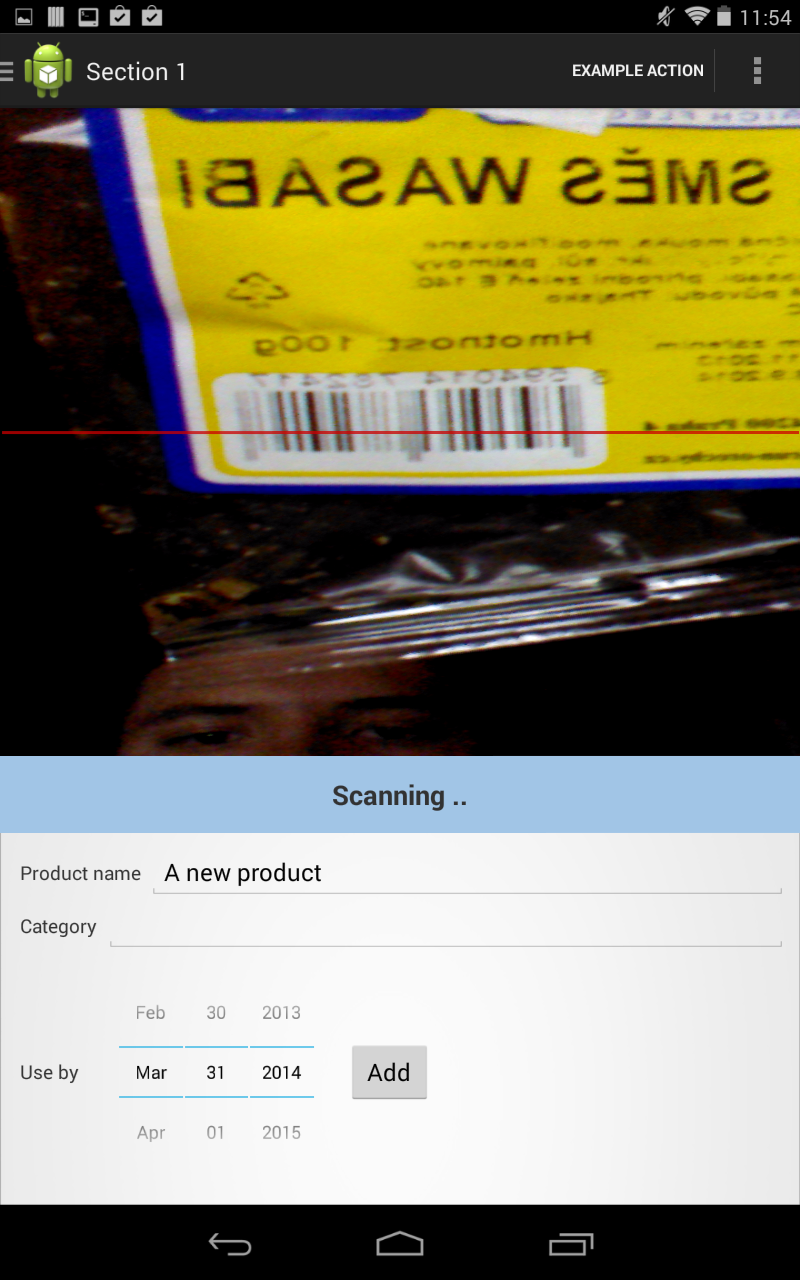
\includegraphics[scale=0.3]{screenshots/scan_prototype.png}
  \caption{Prototyp snímaní čárových kódů}
  \label{fig:ScanPrototype}
\end{figure}

\clearpage

\section{Případy užití}

Výše uvedené funkční požadavky se přimo promítají do případů užití. Tento diagram slouží pří návrhu UI i jako scénáře pro uživatelské testování, které ověří, zda daný návrh je pro uživatele dostatečne jednoduchý a zda-li je uživatel schopen v aplikaci dosáhnout všech daných cílu.

Inventář a vyhledání potraviny jsou základnami, ze kterých se dále odvíjejí ostatní činnosti. Jednotlivé případy vystihují přesně ty činnosti, které bude uživatel provádět během používání aplikace.

Při vytváření tohoto diagramu byl dán veliký důraz na nejčastější činnosti uživatele, které lze očekávat. V závěru práce dojde ke zhodnocení zde navrhnutých scénářů a přípádné návrhy na změnu do budoucnosti.

\begin{figure}[H]
  \centering
  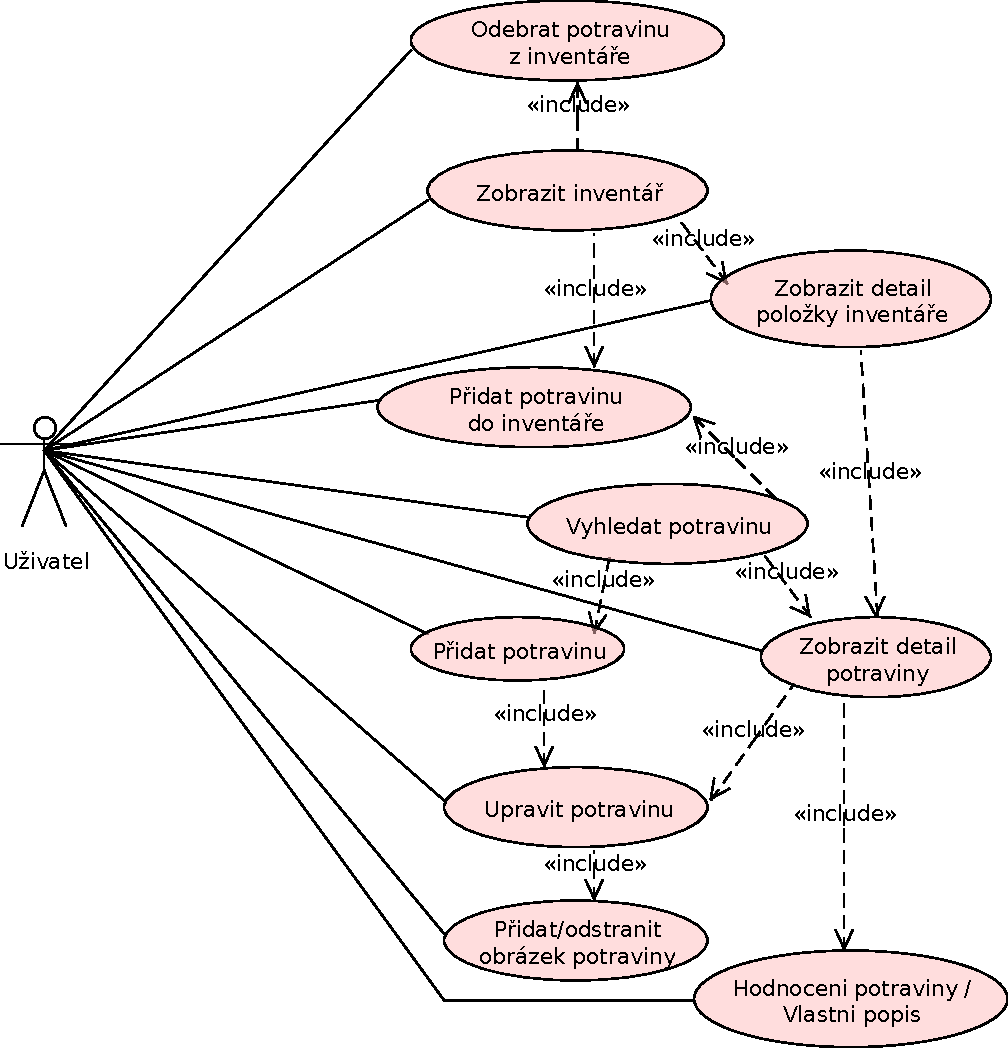
\includegraphics[scale=0.75]{diagrams/use_case}
  \caption{Diagram případů užití}
  \label{fig:UseCase}
\end{figure}

\chapter{Návrh}

Kapitola návrh poskytne soubor informací k následné implementaci. Požadavky sepsány v kapitole Analýza budou pevně diktovat jeho obsah. Struktura návrhu se týka návrhu architektury, doménového modelu, databázového modelu, bussiness modelu, class diagramu a popis komunikačního protokolu.

\section{Architektura}

Vzhledem nutnosti použít pro mobilní aplikaci server bude nejvhodnější model architektury klient - server. Tento model vyžaduje specifikovat komunikaci mezi obouma stranami a dále při vhodném navrhnutí lze uvažovat i o klientech pro více platforem. Vhodná platforma pro jiný typ aplikace by mohla být webová aplikace, která by zpřístupňovala aplikaci na všech ostatních platformách skrze webový prohlížeč. Touto cestou by však nebylo možné uživatele jednoduše upozorňovat o trvanlivosti přímo z webové stránky i v době, kdy uživatel stránku nepoužívá.

\subsection{Klient}

Z nefunkčního požadavku OS Android vyplývá nutnost implementovat aplikaci s pomocí jeho SDK. Existují multiplatformní SDK nabízející bežné API, avšak nutnost vytváření upozornění a snímaní čárových kódů je čistě specifická záležitost pro kažou platformu zvlášť. Tuto možnost autor předpokládá jako časově náročnou, proto se tato práce soustředí pouze na Android SDK.

\subsection{Server}

Jako jeden z hlavních požadavků na server je jeho malý paměťový otisk. Nabízí se spousta různých variant, jak tohoto cíle dosáhnout. Jelikož předměty prvního ročníku autorova studia obsahovali především algoritmizace v jazycích C/C++ a obor softwarového inženýrství si vyžádal předmět efektivních algoritmů, byla jako vhodná varianta serveru jeho implementace v jazyce C++. Bližší detaily jeho návrhu budou priblíženy dále.

\section{Doménový model}

Na obrázku doménovém modelu ~\ref{fig:DomainModel} lze spatřit vztahy mezi všemi entitami, jejichž význam zde bude vysvětlen.

\subsection{Category}
Category poskytuje kategorizaci potravin. Tato entita je připravena pro budoucí rozšíření vyhledávání, v rámci této práce je informace o kategorii pouze shromažďována. 

\subsection{Edit}
Každá editace potraviny tvoří záznam entity Edit, ve které se nachází informace kdo, kdy a co upravil. Tato informace poté může sloužit k blokování škodlivých uživatelů.

\subsection{Food}
Entita food popisuje potravinu.

\subsection{Image}
Každá potravina může nabýt předem nespecifikované množství obrázků od uživatelů.

\subsection{Inventory}
Položka inventáře spojující uživatele a potravinu, která zároveň určuje datum spotřeby. Při přidání několika instancí potraviny do inventáře najednou se vždy přidá stejný počet záznamů této entity.

\subsection{Review}
Jednoduché hodnocení potraviny od 0 do 5 s volitelným textem recenze uživatele. Každý uživatel může nabýt nejvíce 1 hodnocení.

\subsection{User}
Entita uživatele, uchovávající pouze uživatelské jméno. Tuto entitu bude nutné v budoucnu rozšířit o příslušné vlastnosti pokud bude třeba uživatelská data více zabezpečit.

\subsection{Vendor}
Výrobce je specifikován jako samostatná entita, v budoucnu lze také použít pro filtrování vyhledávání stejně jako je tomu u kategorie.

\begin{figure}[H]
  \centering
  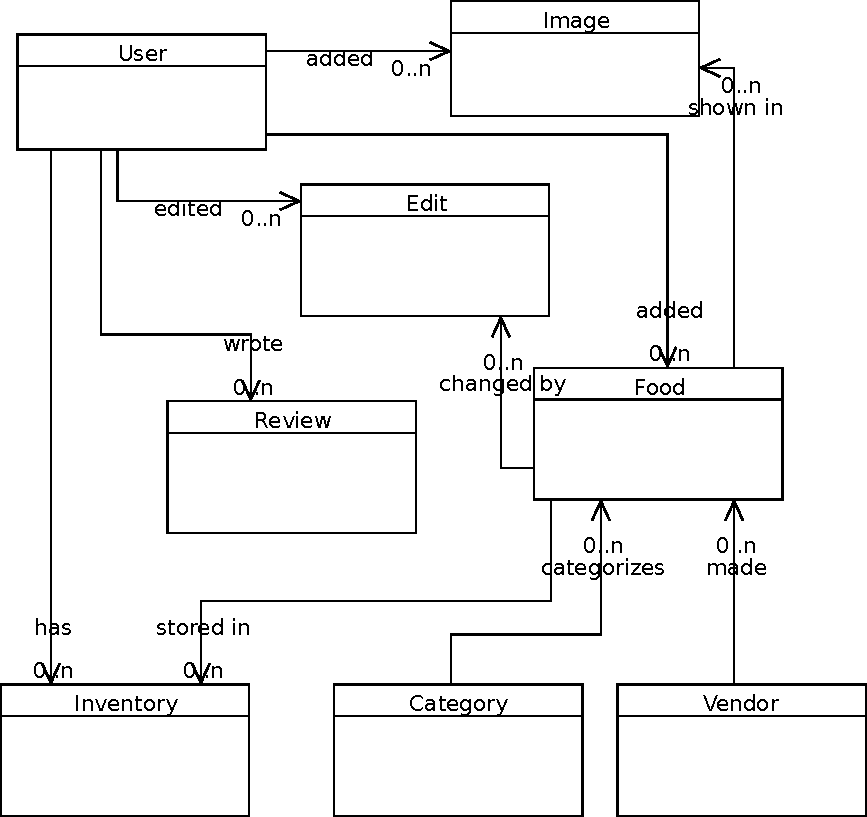
\includegraphics[scale=0.75]{diagrams/model}
  \caption{Doménový model}
  \label{fig:DomainModel}
\end{figure}

\section{Databázový model}

Z protředků cílového stroje určeného k nasazení serveru této aplikace je jako databázový software zvolen MySQL. K návrhu byl využit software MySQL Workbench, který umožnuje vytvořit relační model, který je přímo kompatibilní s vlastnostmi MySQL. Jelikož jsou veškerá data aplikace uchovávána na serveru, vychází relační model přímo z doménového. Entity tedy zůstávají stejné. Detaily jednotlivých entit jsou plně zřetelné z relačního modelu a není třeba je dále rozepisovat.

\begin{figure}[H]
  \centering
  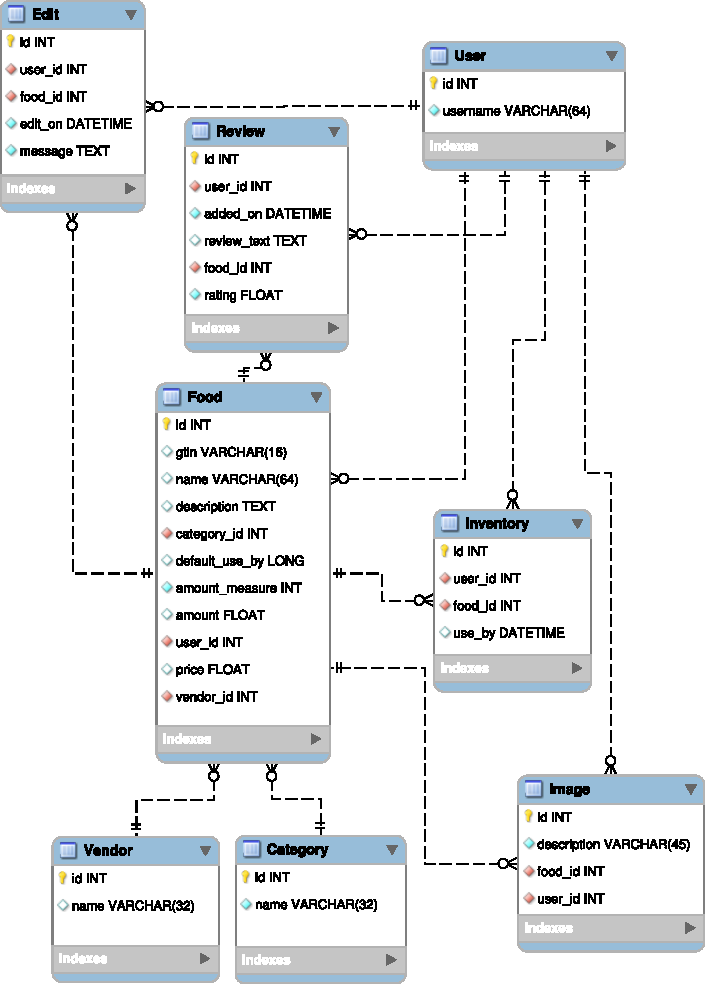
\includegraphics[scale=1.20]{diagrams/relational_model}
  \caption{Relační model}
  \label{fig:RelationalModel}
\end{figure}


\section{Komunikační formát a protokol}

Z důvodu zvolené architektury je nutné specifikovat protokol, jakým budou mezi sebou komunikovat klient a server. Android SDK diktuje pro mobilního klienta použití jazyku Java, který sice lze nahradit pomocí C/C++, toho se však doporučuje jen v aplikací či knihovnách s potřebou vysokého výkonu nebo přístupu k hardware ~\cite{android_ndk}. Tato odlišnost vyžaduje použít platformě nezávislý protokol na bázi například textu.

\subsection{XML}

Mnoho protokolů využíva ke komunikaci textový formát v XML. Tento formát je podobný HTML, je platformě nezávislý a široce podporován. V C/C++ ho implementují různé knihovny, které jsou dostupné jako svobodný software. Protokol však nevyžívá datový prostor dostatečně efektivně, jak bude popsáno dále.

\subsection{JSON}

Jako další textový formát umožňující platformově nezávislý přenos dat je JSON. Je to velice populární formát používaný široce ve webových technologiích a jeho použití je také velmi jednoduché. Formát vychází z JavaScriptové notace a lze ho s bezpečnostními opatřeními načíst jako samotný zdrojový kód JavaScriptu. Výhodou formátu JSON je jeho kompaktnost oproti formátu XML, čímž dojde ke snížení přenášeného množství dat a přesto se zachová textový formát dat.

\subsection{Porovnání a zvolení formátu}

Oba formáty jsou přímo podporovány v Android API a tak jsou vhodnými kandidáty. Od obou formátu jsou k dispozici různé kompaktnější verze, které ještě více data zhušťují nebo využívají jiné kompresní algoritmy pro snížení velikosti jejich dat. Využití takovýchto vylepšení je však omezující jeho podporou různých prostředí a neumožňují lidsky čitelný formát, který je vhodný pro vývoj a odhalování chyb.

Různé knihovny implementují tyto formáty i do C++, které jejich podporu ve standardních knihovnách neobsahuje. Jelikož jediný patrný rozdíl je ve větší kompaktnosti, byl zvolen JSON jako formát protokolu pro tuto aplikaci.

\subsection{Struktura protokolu}

Protokol budou tvořit zprávy, které budou mít pevný tvar. Kvůli možnosti budoucího vylepšení protokolu a jednoduchosti jeho načtení ze síťového proudu je vhodné poslat přesný počet bytů každé zprávy vepvně daném pořadí. Zpráva bude mít teoreticky neomezenou velikost, avšak server bude mít možnost tuto velikost omezit kvůli zabránění zahlcení serveru jednoduchým útokem, který by zaplnil celou dostupnou pamět a způsobil pád serveru. Maximální velikost zprávy bude možné nastavit v serveru a bude také hodnota, která s dalšími vlastnostmi určí maximální množství uživatelů, který je server schopen v extrémním případě obsloužit.

Komunikaci budou tvořit zprávy přenesené v přesném pořadí jako:

\begin{itemize}
  \item{4 byty určující celé číslo N v Big Endian pořadí, stejné jako Network Byte Order}
  \item{N bytů textové UTF-8 zprávy}
\end{itemize}

Zprávy budou mít dále již v JSON formátu strukturu:
\begin{lstlisting}
{
  "header" : "NazevZpravy",
  "content" :
    {
      .. dalsi obsah zpravy ..
    }
}
\end{lstlisting}

\begin{itemize}
  \item{položka header určuje název zprávy, který bude popsán dále}
  \item{položka content obsahuje položky určité zprávy}
\end{itemize}

Zprávy budou mít povahu požadavku a odpovědi na něj. Klient bude posílat serveru požadavky a ten mu na ně příslušně odpovídat. Neznámé zprávy způsobí ukončení komunikace.

Jednotlivé zprávy byly navrženy již s ohledem na funkce uživatelského rozhraní. Tyto zprávy budou dále popsány, jejich pevnou strukturu však bude možné zjistit ze zdrojového kódu, neboť rozsah této práce takovouto specifikaci neumožňuje. Zprávy kromě poslední KeepAlive jsou dvojice Request a Respond, např. pro zprávu Login to je LoginRequest a LoginResponse.

\begin{itemize}
  \item{\textbf{Login} - přihlásí uživatele pod jménem (e-mailem) a vrátí odpověď jako boolean, zda-li tak proběhlo}
  \item{\textbf{GetInventory} - vyhledá a vrátí množinu položek inventáře podle zadaného jména nebo kódu GTIN}
  \item{\textbf{GetFoodDetail} - vratí veškeré detaily potraviny}
  \item{\textbf{GetFoodItem} - vyhledá vrátí množinu potravin podle jména nebo GTIN kódu}
  \item{\textbf{EditInventory} - upraví položku inventáře}
  \item{\textbf{DeleteInventory} - smaže položku inventáře}
  \item{\textbf{EditFood} - upraví detail potraviny}
  \item{\textbf{GetFoodBase} - vrátí podklady k zadání potraviny: výrobce a kategorie}
  \item{\textbf{AddImage} - nahraje nový obrázek potraviny}
  \item{\textbf{DeleteImage} - smaže zadaný obrázek potraviny}
  \item{\textbf{SetUserReview} - nastaví nebo smaže uživatelovu recenzi}
  \item{\textbf{KeepAlive} - příkaz udržující spojení po dobu od posledního}
\end{itemize}

\section{Server}

Z výše uvedených požadavků lze vypsat tyto vlastnosti, které musí server splňovat:

\begin{itemize}
  \item{Implementace v C++}
  \item{Škálovatelnost}
  \item{Zdroj dat z MySQL}
  \item{Implementace protokolu s JSON formátem}
\end{itemize}

Následující podsekce popisují zvolené detaily těchto vlasntostí.

\subsection{C++}

Implementace v C++ se může zdát jako silně platformově závislá. Opak je však pravdou. Pro implementaci serveru byl totiž zvolen ISO C++ standard C++11, který mimo jiné přináší multiplatformní podporu vláknování. Dále také umožňuje tvořit snadněji určité konstrukce, které byly dříve obtížnější. Díky těmto vlastnostem by následná implementace serveru měla být jednodušší, neboť není třeba příliš uvažovat o rozdílech jednotlivých platforem až na vytváření serverového socketu, které je ale velice podobné na všech používaných platformách a jeho přizpůsobení je tím pádem velice jednoduché.

\subsection{Škálovatelnost}

Aby bylo možné server přizpůsobit výkonějšímu hardware, je třeba příslušné škálovatelnosti. V případě této práce se jako její nejjednodušší forma jeví použití vlákna pro každého připojeného uživatele zvlášť. Je však také nutné zajistit, že další prostředky jako například připojení k databázi bude pro vlákna dostupné soubežně a tím umožní zpracovávat více databázových dotazů současně. Je to důležite zejména proto, že tyto operace jsou obecně časově nejnáročnější. Tato forma škálovatelnosti však umožní získat vyšší výkon pouze za předpokladu, že dojde ke zvýšení počtu výpočetních jednotek, které mohou provádět instrukce jednotlivých vláken současně.

Jako další forma škálovatelnosti se již nabízí pouze přizpůsobení větší dostupné dynamické paměti. Zde jde třeba zdůraznit, že navrhnutý komunikační protokol vyžaduje určitou paměťovou režii kvůli dále zmíněné knihovně pro podporu JSON. Server tedy bude mít možnost upravit maximální počet současně obshluhovaných uživatelů, které bude závislé na dostupné paměti.

\subsection{MySQL}

Pro pohodlné a jednoduché použití MySQL v C++ je vhodné využít rozhraní jiné než poskytované samotnou klientskou knihovnou. Jako vhodná multiplatformní knihovna poskytující takové rozhaní se jeví MySQL Connector/C++. Tato knihovna nabízí rozhraní velmi podobné s tím, co je dostupné pro použití v jazyce Java - lze tedy použít například PreparedStatement, které ošetří případné útoky pomocí pokoření formátu dotazů a podobné. Dále poskytuje vyjímky pro běžné chyby, které mohou nastat v rámci jejího použití. Je tedy vhodná pro objektový návržený server. Kromě těchto vlastností umí také poskytovat více připojení k samotnému databázovému serveru, takže poskytne vyžadovanou škálovatelnost z podsekce výše.

\subsection{JSON}

Knihoven podpory JSON pro použití jazykem C++ je mnoho. Po delším uvažování byla vybrána knihovna JsonCpp. Tato umožňuje použití prvků formátu JSON jako objekty a výrazně tak zjednodušit jejich integraci do serverové aplikace. Knihovna je také multiplatformní.

Při testování zmíněné knihovny JsonCpp však vyšlo najevo, že knihovna nepoužívá vyjímky pro zachycení nejrůznejších chyb. Některé chyby způsobily přímo pád serverové aplikace. Tuto vlastnost tedy bylo třeba povolit. Tato úloha se však ukázala jako velmi jednoduchá. Jelikož zkompilovaná verze, která je bežně dostupná, vyjímky nevyhazuje, je třeba do serveru přidat počateční test, který ověří, zda-li je možné odchytit chyby při použití této knihovny a v případě, že tomu tak není následně upozorní uživatele.

Pro podporu vyjímek byl zřízen speciální repozitář~\cite{json_ex_repo} s aplikovaným patchem pro tuto vlastnost. Použití této upravené verze je tedy nutnost pro bezchybný běh serveru.

\subsection{Návrh tříd}

Protože návrh tříd je příliš rozsáhlý, není vhodné ho zde prezentovat. Detailnější informace jsou dostupné v rámci hlavičkových souborů v poskytnutých zdrojových kódech k této práci.

Třídy serveru však lze rozlišit na základní kategorie, které také učí kořenovou strukturu zdrojových kódů:

\begin{itemize}
  \item{\textbf{Client} - třídy pro obsluhu klientů}
  \item{\textbf{Config} - třídy poskytující nastavení serveru}
  \item{\textbf{Database} - obsluha připojení do databázového serveru a implementace jednotlivých tříd poskytujících správu entit}
  \item{\textbf{Entity} - třídy jednotlivách entit a rozhraní jejich správy}
  \item{\textbf{Handler} - třídy pro obsluhu příkazů ze zpráv komunikace}
  \item{\textbf{Network} - třídy socketového serveru}
  \item{\textbf{Protocol} - třídy zpráv}
  \item{\textbf{Util} - obecné a pomocné třídy}
\end{itemize}

\section{Klient}

Jelikož klient této aplikace slouží jako rozhraní pro uživatele, je třeba dbát na návrh uživatelského rozhraní co nejvíce. Návrh klienta dále popisuje další klíčové oblasti, které je nutné správně navrhnout.

\subsection{Uživatelské rozhraní}

Při návrhu bylo dbáno především na požadavek jednoduchosti. Tvorba uživatelského rozhraní je možná v různém softwaru. V případě OS Android je však návrh proveditelný přímo do spustitelné podoby s pomocí vývojářských nástrojů. Tento postup s sebou přínáší následující výhody:

\begin{itemize}
  \item{Jednoduchost návrhu - nástroje velmi intuitivní}
  \item{Nástroje umožňují předem získat přehled o vzhledu na různých typech obrazovek}
  \item{Vytvořený návrh lze okamžitě testovat mezi dobrovolníky zasláním aplikace}
  \item{Výsledná podoba návrhu již nemusí být vytvářena znova a lze využít již hotový návrh}
\end{itemize}

Dále jsou popsány jednotlivé obrazovky zajímavé pro uživatele.

\subsubsection{Menu}

První obrazovkou, kterou uživatel po spuštění aplikace uvidí, je toto ~\ref{fig:AppMenu} menu. Je přímo dostupné ze všech cílu položek tohoto menu stiskem tlačítka v horní levé části nebo posunutím ukazatele (prstu) od okraje obrazovky do jejího středu. Z ostatních podpoložek se lze dostat zpět standardně tlačítkem zpět, případně tlačítkem v horním panelu, tzv. ActionBaru.

Důvod existence pouze těchto položek spočívá v jednoduchosti navigace. Scénář použití vždy začíná v jedné z těchto položek. Nastavení je standardně přes stisk klávesy menu nebo přes ikonu menu v ActionBaru, proto není zbytečně umístěno také zde. Stejné je to s nastavením i na ostatních obrazovkách.

\begin{figure}[H]
  \centering
  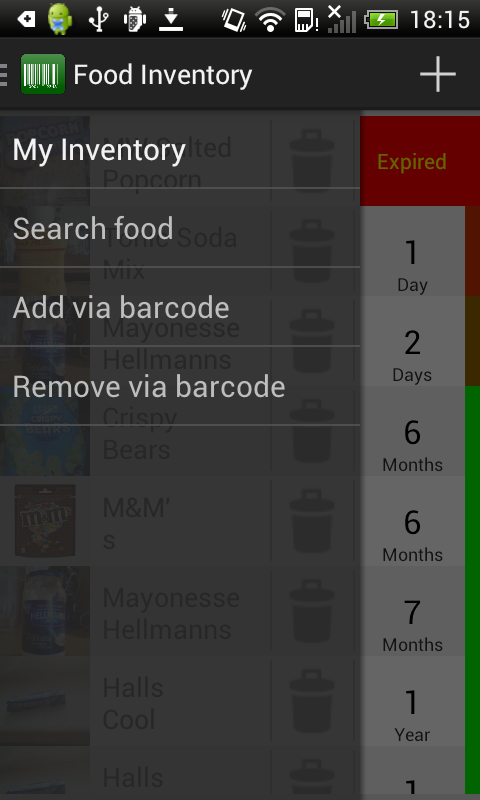
\includegraphics[scale=0.4]{screenshots/app_menu.png}
  \caption{Menu aplikace}
  \label{fig:AppMenu}
\end{figure}

\clearpage

\subsubsection{Inventář}

Inventář se stejně jako menu zobrazí při prvním spuštění, avšak zůstane v jeho pozadí. Zachycuje ho obrazovka ~\ref{fig:AppInventory}. Lze zde pozorovat seznam potravin, který vlastní uživatel. Tyto položky inventáře dále disponují datumem spotřeby, díky kterému docházi k seřazení a následně je u potravin barevně vyznačen jejich status trvanlivosti. Červeně jsou vyznačeny potraviny s končící trvanlivostí a postupně přechodem do zelené ty, které jsou od konce trvanlivosti vzdáleny více než týden.

Každá položka inventáře reaguje na stisk uživatelem. Při stisku dojde k zobrazení detailu položky, který je popsán dále. Pro odebrání je k dispozici ikona odpadkového koše, který potravinu z inventáře odstraní.

Přidání nové položky do inventáře bude nejpravděpodobnější činností nového uživatele, proto je na horním panelu tlačítko plus, které zobrazí dialog pro zvolení, zda-li potravinu načíst čárovým kódem nebo ji vyhledat manuálně. Nahrazuje tím v podstatě část menu aplikace. Je tu zde však pouze pro úplnost, aby noví uživatelé nebyli příliš zmateni z prázdného seznamu, který se po prvotním spuštění ukáže.

\begin{figure}[H]
  \centering
  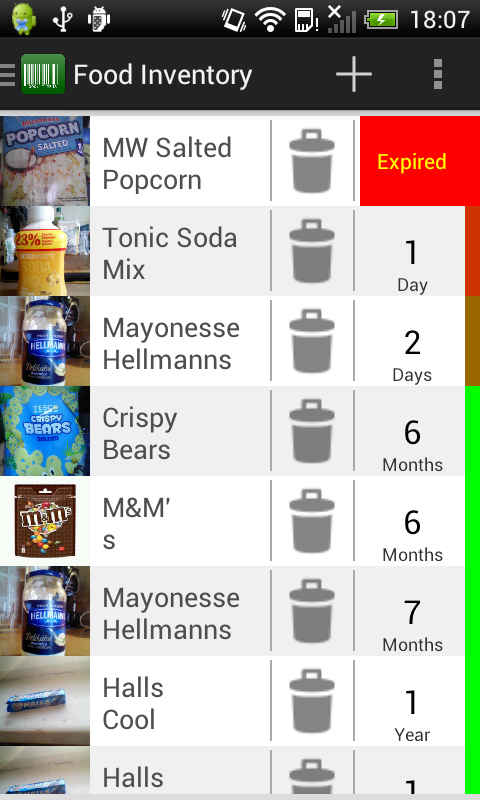
\includegraphics[scale=0.4]{screenshots/app_inventory.png}
  \caption{Inventář}
  \label{fig:AppInventory}
\end{figure}

\clearpage

\subsubsection{Detail inventáře}

Obrazovka~\ref{fig:AppInventoryDetail} zobrazená po stisku položky inventáře ukazuje dialog obsahující detail položky inventáře, kde lze upravit datum spotřeby a případně přejít na detail potraviny, která je položkou tohoto inventáře. Při navigaci zpět zůstává dialog zobrazený stejně jako změny provedené uvnitř.

Tlačítky Ok a Cancel lze uložit či zrušit zvolenou změnu datumu. Uložení způsobí nové stahnutí položek inventáře ze serveru.

Samotné načítaní inventáře probíhá za zobrazení standardního ukazatele průběhu, který je schován spolu s plně načteným inventářem a jeho zobrazením.

\begin{figure}[H]
  \centering
  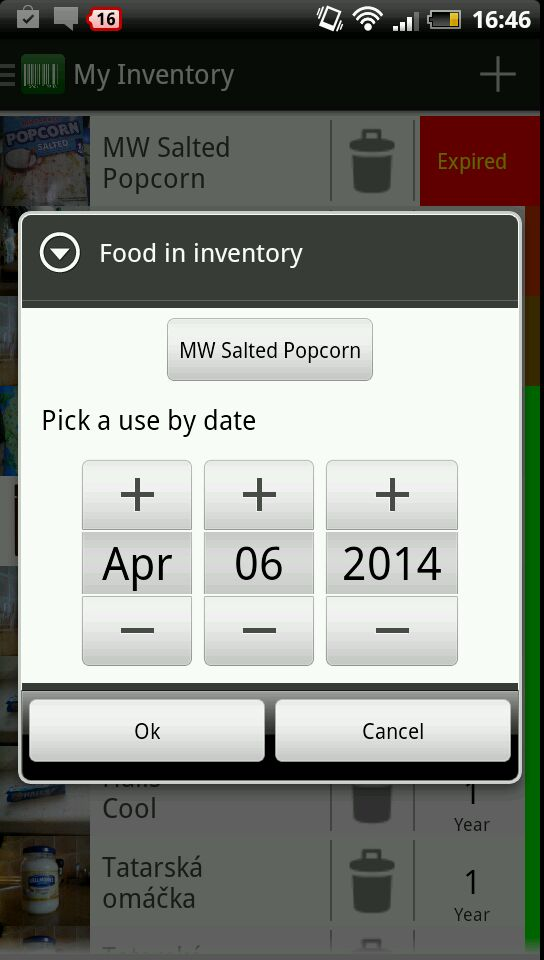
\includegraphics[scale=0.4]{screenshots/app_inventory_detail.jpg}
  \caption{Detail inventáře}
  \label{fig:AppInventoryDetail}
\end{figure}

\clearpage

\subsubsection{Vyhledávání potravin}

Z menu nebo z tlačítka přidání v inventáři se uživatel může dostat do obrazovky vyhledání potravin~\ref{fig:AppSearch}. Pro vyhledávání je zde přítomen jeden jediný textové políčko, které napovídá uživateli, že může vyhledávat pomocí jména potraviny či jejího čárového kódu.

Při psaní textu do políčka vyhledávání je dále zobrazována nápověda jako seznam potravin, které by byly zobrazeny při aktuálním textu v políčku po stisku klávesy. Pokud uživatel na položku nápovědy klikne, vybraný text se vyplní do políčka.

Pro samotné vyhledání podle políčka stiskne uživatel klávesu Search, která zobrazí obrazovku~\ref{AppSearchResults}.

V této obrazovce je do budoucna dále možné uvést filtraci výsledků pomocí jména výrobce, kategorie či jiných parametrů, které jsou již navrženy v aktuálním databázovém modelu.

\begin{figure}[H]
  \centering
  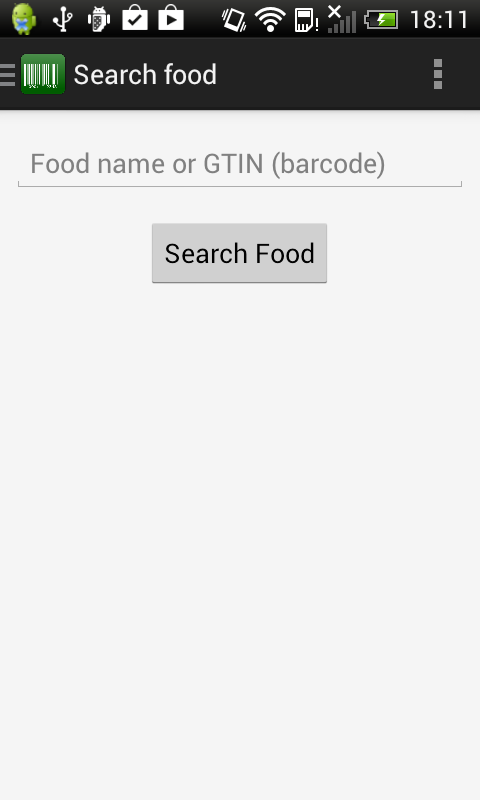
\includegraphics[scale=0.4]{screenshots/app_search.png}
  \caption{Vyhledávání potravin}
  \label{fig:AppSearch}
\end{figure}

\clearpage

\subsubsection{Seznam výsledků hledání potravin}

Tato obrazovka~\ref{fig:AppSearchResults} zobrazena po vyhledávání v obrazovce~\ref{fig:AppSearch} zobrazuje seznam nalezených výsledků. Při probíhajícím vyhledávání je seznam nahrazen prvkem ukazující probíhající činnost, který je zpět schován a zobrazen seznam výsledků při dokončení.

V tomto seznamu výsledků se v pravém horním rohu nabízí tlačítko plus, které umožní uživateli přidat novou potravinu, neboť je to místo, kde uživatel zjistí, že taková to potravina neexistuje. Přidání potraviny potom probíha stejně jako při editaci~\ref{fig:AppFoodEdit}.

V seznamu výsledků je dále možné zobrazit detail potraviny~\ref{fig:AppFoodDetail} nebo přidání této potraviny do inventáře stisknutím tlačítka plus, které se nachází napravo v položce seznamu. Toto stisknutí zobrazí dialog~\ref{fig:AppScanAddFood}.

\begin{figure}[H]
  \centering
  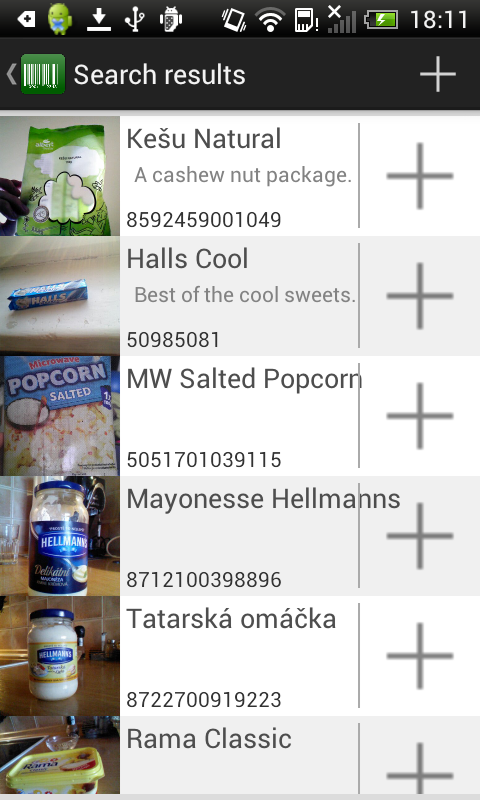
\includegraphics[scale=0.4]{screenshots/app_search_results.png}
  \caption{Seznam výsledků hledání potravin}
  \label{fig:AppSearchResults}
\end{figure}

\clearpage

\subsubsection{Přidání potraviny do inventáře}

V tomto dialogu~\ref{fig:AppScanAddFood} je zobrazen název potraviny, výběr datumu spotřeby a počet takových kusů. Každý takový kus bude přidán jako jedna položka inventáře.

Stisk tlačítka s názvem potraviny uživatele přesune do detailu potraviny~\ref{fig:AppFoodDetail}, ze kterého se navigací zpět dostane zpátky do tohoto dialogu.

Tento Dialog se zobrazuje při přidávání z výsledků hledání potravin i ze čtení čárového kódu za tímto účelem.

\begin{figure}[H]
  \centering
  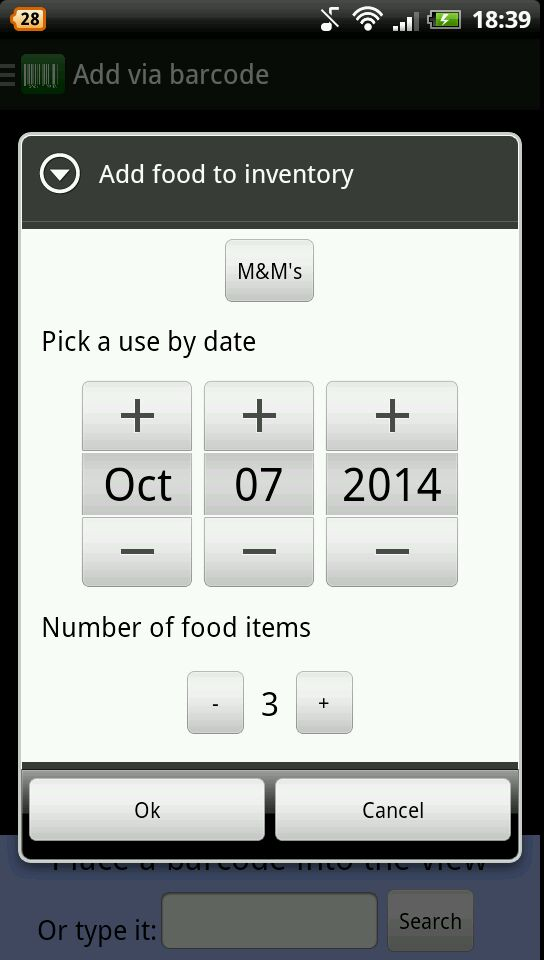
\includegraphics[scale=0.4]{screenshots/app_scan_add_food.jpg}
  \caption{Dialog přidání potraviny do inventáře}
  \label{fig:AppScanAddFood}
\end{figure}

\clearpage

\subsubsection{Detail potraviny}

Obrazovka~\ref{fig:AppFoodDetail} ukazuje částečný detail potraviny. V tomto místě je možné si potravinu detailnějí prohlédnout a hodnotit. Také z této obrazovky lze potravinu upravit pomocí tlačítka tužky v pravém horním rohu.

Hodnocení potraviny probíha pomocí dialogu, který se dotáže na číselné ohodnocení spolu s volitelným textem recenze. Pro uložení uživatel stiskne tlačítko Rate, v opačném případě uživatel stiskne delete, který odstraní hodnocení, pokud existuje. Každý uživatel může potravinu hodnotit maximálně jednou.

Ve spodní části jsou dále vidět 2 uživatelé. První je ten, kdo potravinu přidal jako první a druhý ten, kdo potravinu naposledny upravil.

\begin{figure}[H]
  \centering
  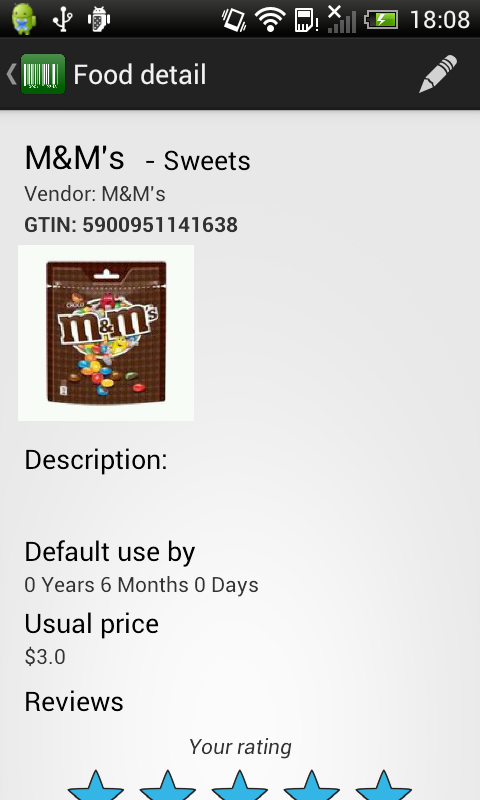
\includegraphics[scale=0.4]{screenshots/app_food_detail.png}
  \caption{Detail potraviny}
  \label{fig:AppFoodDetail}
\end{figure}

\clearpage

\subsubsection{Editace potraviny}

K editaci potraviny slouží obrazovka~\ref{fig:AppFoodEdit}. Stejně tak slouží i pro přidání potraviny pouze s tím, že všechny položky jsou nastavené na výchozí hodnoty nebo hodnoty takové, které se porařilo zajistit jiným způsobem. Zde je možné nastavit jméno, výrobce i předem určené obecně uznávané kategorie potravin, čárový kód, obrázky potraviny, hmotnost nebo objem a výchozí datum spotřeby.

Výber kategorie i výrobce poskytuje dialog. Pro výrobce je však možné určit název manuálně, čímž dojde k přidání výrobce do seznamu všech.

Nastavení čárového kódu je možné buď manuálně, či je vedle něj tlačíkto, které zobrazí stejnou obrazovku jako při přidání potraviny~\ref{fig:AppScanAdd}, která po načtení čárového kódu zanikne a vyplní číslo čárového kódu tím načteným.

Obrázky je možné přidávat tlačítkem Add image a mazat pomocí tlačítka delete již existující obrázky.

Pro samotné uložení změn potraviny (nebo vytvoření nové) slouží tlačítko v podobě diskety v pravém horním rohu na panelu ActionBar. Uložení proběhne se zobrazeným dialogem průběhu, neboť nahrávání obrázků může trvat delší dobu.

\begin{figure}[H]
  \centering
  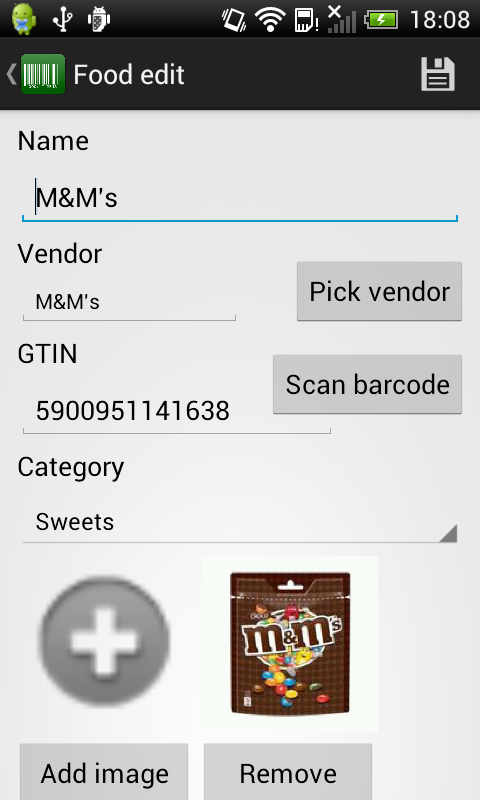
\includegraphics[scale=0.35]{screenshots/app_food_edit.png}
  \caption{Editace potraviny}
  \label{fig:AppFoodEdit}
\end{figure}

\clearpage

\subsubsection{Přidání potraviny do inventáře čárovým kódem}

Pro samotne přidání potraviny pomocí čárového kódu slouží obrazovka~\ref{fig:AppScanAdd}. Uživatel je pobídnut k položení čárového kódu do náhledu kamery. Pokud dojde k úspěšnému načtení, spustí se vyhledání potraviny na serveru, které je signalizováno dialogem pruběhu.

V případě úspešného nalezení potraviny se zobrazí dialog pro přidání potraviny~\ref{fig:AppScanAdd} stejný jako v případě manuálního hledání potraviny. Po zrušení dialogu či jeho potvrzení se vrátí obrazovka načítaní čárového kódu, aby mohla být načtena další potravina.

Pokud však potravina naleznuta nebyla, spustí se dále hledání v externí databázi, které bude popsáno dále v této sekci. Signalizováno je také pomocí dialogu průbehu. Při nalezení či nenalezení v externi databázi se zobrazí dialog, který buď pobízí vytvoření nové potraviny s importem nalezených informací~\ref{fig:AppScanAddImport} nebo k pouhému vytvoření nové potraviny. Do té bude přenesen načtený kód nebo další informace získané z externí databáze. Přidání potraviny probíhá stejně jako při jejím vytváření při vyhledávání. Po přidání či odmítnutí přidání potraviny se znovu zobrazí obrazovka pro načtení čárového kódu, aby mohl uživatel dále pokračovat v načítání.

\begin{figure}[H]
  \begin{minipage}{0.5\linewidth} 
    \centering
    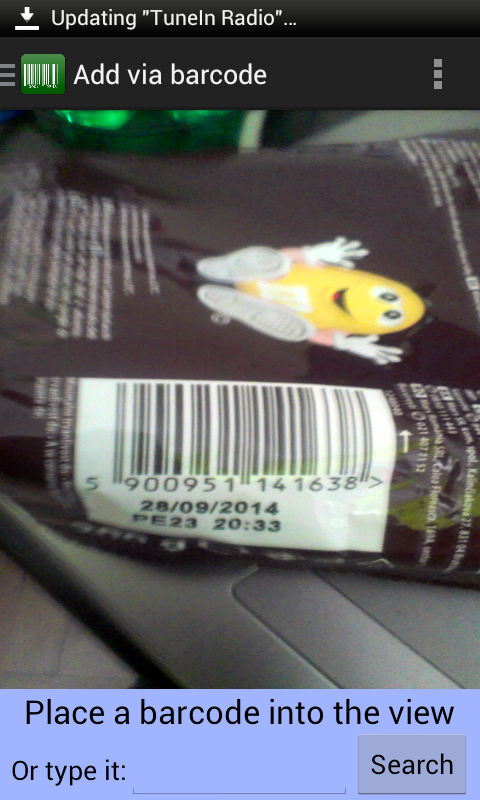
\includegraphics[scale=0.3]{screenshots/app_scan_add.png}
    \caption{Skenování čárového kódu pro přidání potraviny}
    \label{fig:AppScanAdd}
  \end{minipage}
  \begin{minipage}{0.5\linewidth} 
    \centering
    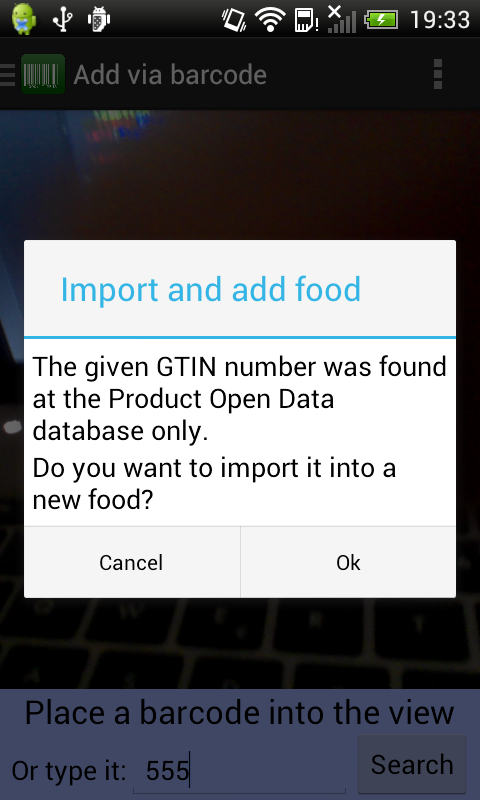
\includegraphics[scale=0.3]{screenshots/app_scan_add_import.png}
    \caption{Import informací z externí databáze Product Open Data}
    \label{fig:AppScanAddImport}
  \end{minipage} 
\end{figure}

\clearpage

\subsubsection{Odebrání potraviny z inventáře čárovým kódem}

Podobně jako obrazovka pro načtení čárového kódu pro přidání potraviny~\ref{fig:AppScanAdd} vypadá i tato pro její odebrání z inventáře.

Při načtení čárového kódu dojde k vyhledání v uživatelově inventáři a zobrazení seznamu potravin ~\ref{fig:AppScanRemoveList}, který je stejný jako z obrazovky zobrazení celého inventáře ~\ref{fig:AppInventory}. Smazání položky seznamu tedy probíha stejně.

\begin{figure}[H]
  \centering
  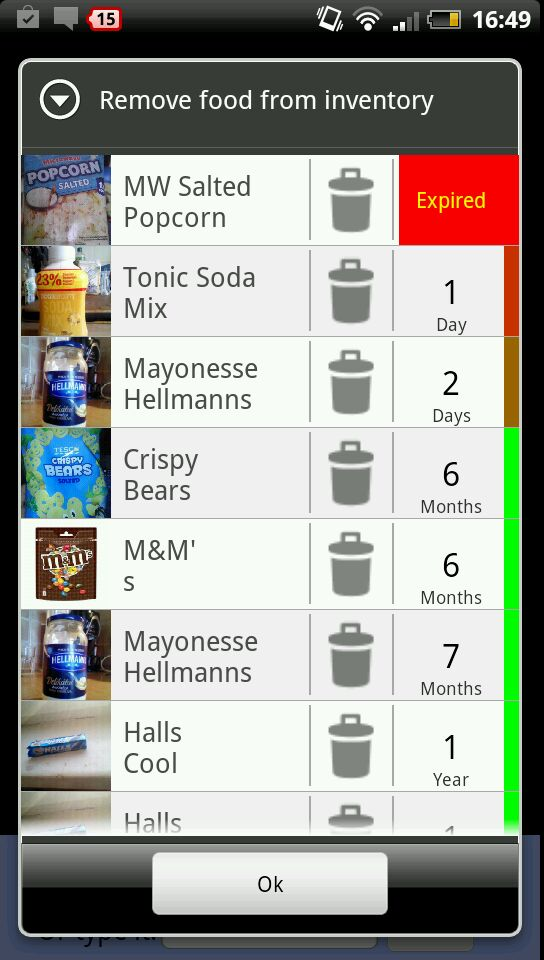
\includegraphics[scale=0.4]{screenshots/app_scan_remove_list.jpg}
  \caption{Seznam naleznutých potravin s daným čárovým kódem}
  \label{fig:AppScanRemoveList}
\end{figure}

\clearpage

\subsubsection{Nastavení}

Pro změnu volitelných vlastností aplikace slouží obrazovka ~\ref{fig:AppInventoryDetail}.

Zde je možné změnit účet uživatele, zakázat stahování obrázků potravin, povolit notifikace a jejich časování.

Zmíněna je zde také verze spolu s autorem aplikace.

\begin{figure}[H]
  \centering
  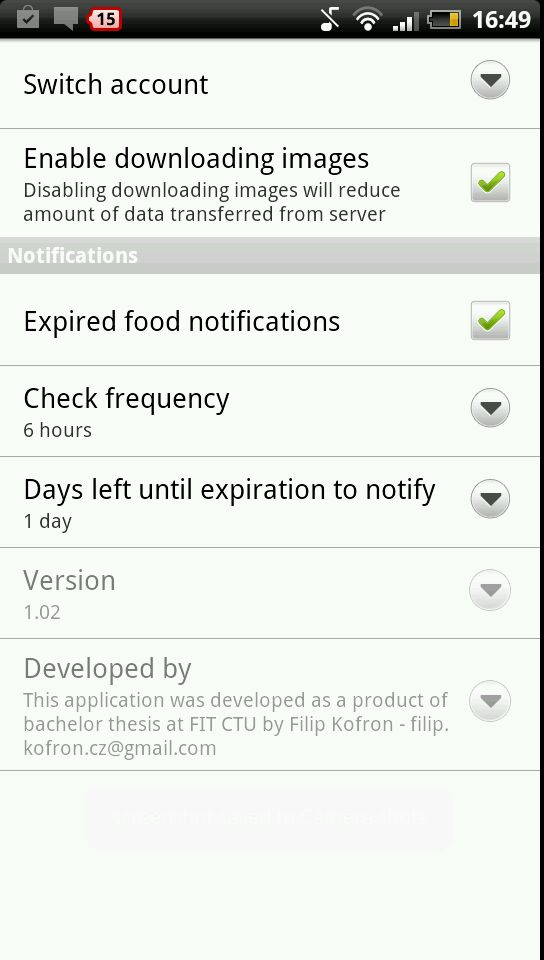
\includegraphics[scale=0.4]{screenshots/app_settings.jpg}
  \caption{Nastavení}
  \label{fig:AppSettings}http://pastebin.com/pU8w3au2
\end{figure}

\clearpage

\subsection{Identifikace uživatele}

Uživatel je identifikován pomocí jména, které si vybere při prvním spuštění aplikace nebo z položky nastavení. Toto jméno je získáno z účtů uživatele v jeho Android. Použito je pouze takové, které je zároveň emailová adreesa a je tím pádem i unikátní.

Vzhledem k jednoduchosti aplikace a nízkému nebezpečí zneužití dat uživatele nevyužije aplikace žádné zabezpečení uživatelova účtu. Pokud se však aplikace stane v budoucnu terčem útoku zvenčí, bude toto vyžadováno.

\subsection{Vyhledávání čárového kódu v externí databázi}

Databáze potravin této aplikace bude ze začátku neobsahovat žádné potraviny. Jelikož může být přidání nové potraviny pro uživatele otravné, je vhodné najít cestu, která by zadávání přinejmenším zjednodušila nebo zcela nahradila.

Jednotlivé potraviny výrobců však není jednoduché získat. Díky zaznamenávání potravin pomocí GTIN kódu se však nabízí možnost získat informace o potravinách z veřejné a otevřené databáze produktů POD - Product Open Data~\cite{pod}. V této databázi je možné k začátku roku 2014 nalézt stovky tisíců záznamů. Informace v databázi obsahují u některých potravin složení, ale u některých naopak pouze jejich výrobce. Možství dat, které se při náhodné analýze této databáze podařilo získat, bylo nedostatečné pro vyplňění většiny potravin. Je zde však možnost využít i pouze částečné informace a ty k potravině doplňit.

\subsubsection{Připojení k Product Open Data}

Databázi Product Open Data zpřístupňují online v době psaní toho textu 3 různé projekty. Jedná se o:
\begin{itemize}
  \item{LSA - http://www.pod.lsa-conso.fr/}
  \item{Mingle IO - https://mingle.io/explore?f=product}
  \item{OpenDataSoft - http://pod.opendatasoft.com/explore/}
\end{itemize}

Projekty Mingle IO a OpenDataSoft spojuje podobné API, se kterým lze komunikovat ve formátu JSON, pomocí kterého se lze dotazovat na čárové kódy.všech produktů v databázi. Projekt LSA je pouze webový vyhledávač.

Mezi OpenDataSoft a Mingle IO nebylo příliš rozdílů, kterými by bylo možné vybrat ten vhodnější. Autor tím pádem zvolil projekt, který se zdál být lépe zdokumentovaný a tím pádem snadnější na implementaci, čímž byl projekt OpenDataSoft.

\subsubsection{Integrace v aplikaci}

Integrování vyhledávání v této externí databázi je, jak již bylo zmíněné v návrhu uživatelského rozhraní, pouze dodatečné vyhledání při nenalezeném produktu, který doplňí podporované informace z produktu do vytvářené potraviny. U testovaných potravin v domácnosti autora této práce bylo nalezeno pouze nepatrné množství potravin, u kterých navíc bylo uvedeno pouze jméno a obrázek. I takto základní informace však usnadnila přidávání.

\chapter{Implementace}

Tato kapitola popisuje implentaci navrženého serveru a aplikace. Cílem této kapitoly není detailně popsat implementaci, nýbrž snaha popsat vývojové prostředí, zajímavosti a problémy, které se v průběhu práce vyskytly. Nakonec bude popsán průběh testování a jeho souhrn poznatků.

\section{Vývojové nástroje}
V této sekci lze nalézt všechny použité nástroje při implementaci.

\subsection{Verzovací software a repozitář}

Jelikož byl vývoj uskutečňován na více zařízeních, bylo třeba zajistit vhodné sdílení materiálů a kvůli správě změn také verzování. Jelikož autor již déle používa software Mercurial~\cite{hg}, bylo vhodné, aby pro tuto práci vyzkoušel konkurenční Git~\cite{git}. Oba tyto verzovací nástroje jsousi navzájem velmi podobné s tím rozdílem, že se jen trochu odlišněji ovládají.

Pro sdílení všech materiálů této práce byl zvolen veřejný repozitář pomocí~\cite{repo} služby Github~\cite{github}.

\subsection{Správa a úpravy databáze}

Jako nástroj pro správu databáze byl pro jeho jednoduchost použit řádkový klient dodávaný spolu s MySQL. Některé úpravy však byli prováděny v softwaru PhpMyAdmin~\cite{phpmyadmin} v případech, kdy byl řádkový klient nevhodný či nedostačující. Výhodou PhpMyAdmin je běh z webového prohlížeče, a tak bylo možné upravovat databázi i bez přístupu k příkazové řádce.

\subsection{Prostředí pro klienta v Android OS}

Pro tvorbu klienta pro Android OS se jevilo jako vhodné vývojové prostředí Android Studio ~\cite{android_studio}. Tento software umožňuje návrh uživatelského rozhraní, používat známý verzovací sooftware. Díky jeho multiplatformnosti mohl autor aplikaci vyvíjet v různých operačních systémech.

\subsection{Prostředí pro server}

Implementace serveru probíhala ve vývojovém prostředí QT Creator~\cite{qtcreator}. Důvod výběru tohoto prostředí byla multiplatformnost a podpora multiplatformního sestavovacího systému CMake~\cite{cmake}, kterým byla popsána celá stromová struktura zdrojového kódu serveru. Díky tomuto 

\section{Server}

Jako první částí implementace byl vytvořen základ serveru. Zdrojový kód byl rozdělen do sekcí, ke kterým byla přiřazena stejnojmenná složka. Sekce tvoří následující seznam:
\begin{itemize}
	\item{Client}
	\item{Config}
	\item{Database}
	\item{Entity}
	\item{Handler}
	\item{Network}
	\item{Protocol}
	\item{Util}
\end{itemize}

Tyto sekce jsou sestavovány rekurzivně pomocí zmíněného CMake. Níže jsou jednotlivé sekce popsány. 

\subsection{Client}
Název Client může být zavádějící, neboť tato sekce ve skutečnosti není klient, ale pouze soubory týkající se spojení s klientem. Zde dochází k přijímaní zpráv serveru a k ošetřování chyb, které mohou nastat při komunikaci s klientem. Mezi ně patří i chyby ze strany serveru.

Důležité pro tuto sekci je, aby nemohlo dojít k pádu server. Jelikož server používá spoustu vyjímek, je zde pokryto velké množství těch, které lze odchytnout a které by za určitých okolností způsobily pád serveru.

\subsection{Config}
Zde jsou umístěny soubory pro načítání konfigurace a pro jejich získání za běhu serveru. Konfigurace používá formát JSON a při neposkytnutí konfiguračního souboru jsou nastaveny výchozí hodnoty použité pro lokální testování, které server znepřístupňuje veřejnosti.

\subsection{Database}
V sekci Database jsou implementovány všechny DAO rozhraní, které jsou popsány níže v podsekci Entity. Jejich implementace využívá MySQL Manager, který je také umístěn v této sekci. Jeho úkolem je udržovat již existující a neaktivní spojení do databázového serveru, tím recyklovat jejich instance pro další použití novými požadavky klientů. Toto je velmi důležité, neboť připojení na server je časově náročná operace, jak se ukázalo v průběhu implementace a testování.

\subsection{Entity}
Každá entita doménového modelu vlastní třídu podobného jména obsahující její atributy. Dále jsou zde umístěny všechny rozhraní DAO objektů, které každé entitě přiřazují množinu databázových operací.

\subsection{Handler}
Pro každou zprávu je v sekci Handler umístěna shodně pojmenovaná obslužná třída, která dle přijaté zprávy dále zpracovává klientské požadavky a sama se postará o jeho zaslání zpět v podobě odpovědi.

\subsection{Network}
Soubory síťového socketu serveru a soubory pro uskutečnění odesílání i přijímání dat jsou umístěny v sekci Network. 

\subsection{Protocol}
Každá zpráva kromě zmíněné zprávy KeepAlive obsahuje požadavek a odpověd. Jejich popis atributy je popsán v sekci Protocol.

\subsection{Util}
Pro jednodušší práci s časovými daty, pro testování a debugování byla vyotvořena sekce Util, kde se nalézají všechny zbylé třídy, které přimo nesouvisí s ostatními sekcemi.

Detailní implementace všech částí serveru probíhala průbežně s aplikací podle požadavků, které kladla funcionalita UI. Výhodou souběžné implementace bylo možné jednodušší přizpůsobení obou stran.

\section{Klient}

Implementace klientské aplikace tvořila 2 části:

\begin{itemize}
	\item{Vytvoření síťové vrstvy, která nezasahovala ještě do návrhu uživatelského rozhraní a sloužila také zároveň k testování počínající implementace serveru. Byl pro to vytvořen projekt TestClient, který lze nalézt ve zdrojových kódech této práce.}
	\item{Implementace samotné funkcionality UI a napojení síťové vrstvy. Tato část bude níže rozepsána.}
\end{itemize}

\subsection{Struktura zdrojového kódu}

Struktura klientské aplikace je poněkud rozsáhlejší, proto při popisu jednotlivých částí (zde balíků) jsou části přímo spojené s uživatelským rozhraním seskupeny, jak ukázuje následující seznam:

\begin{itemize}
	\item{Model}
	\item{Adapter}
	\item{Network}
	\item{Task}
	\item{Barcode}
	\item{Util}
	\item{Cache}
	\item{UI prvky - Activity, Fragment, Dialog, Preference, View}
	\item{Background}
\end{itemize}

Každá část je dále detailněji popsána jako v případě serveru. Autor by rád zdůraznil, že tyto části jsou pouze kořenové složky balíku celé aplikace (mimo využité knihovny), a proto ve zdrojovém kódu lze nalézt více podčástí. V rozsahu této práce není možné popsat každou třídu balíků vzlášť, neboť jich aplikace i server obsahují velmi mnoho. Pro více informací o každé části je třeba navštívit přímo zdrojový kód.

\subsubsection{Model}

Entity využité v klientské části aplikace jsou umístěny v této části.

\subsubsection{Adapter}

Některé části uživatelského rozhraní pro zobrazení dat vyžadují adaptery~\cite{adapter} - třídy, které zprostředkovávají jednotlivé prvky dat, které UI prvky pomocí těchto adapterů přimo získávají a následně prezentují uživateli. 

Adapterů je v této aplikaci více, proto jim byla věnována samotná část.

\subsubsection{Network}

Síťová komunikace byla převzata z projektu TestClient uvedeného dříve. Stará se o příjem a odesílání syrových dat po síťi, stejně jako vytváření a udržování spojení.

\subsubsection{Protocol}

Požadavky a odpovědi, které tvoří zprávy v komunikaci, zde mají svou stejnou reprezentaci jako v případě serveru.

\subsubsection{Task}

Každá operace trvající déle či operace, která vyžaduje komunikaci po síti, je potomkem třídy AsyncTask~\cite{async_task} z Android API. Pomocí implementací potomků této třídy lze jednoduše vytvářet asynchronně probíhající úlohy, jejichž hlavní předností oproti vláknům je zabudovaná synchronizace před spuštěním a po dokončení s hlavním vláknem, jež je nutné pro přístup k prvkům UI.

\subsubsection{Barcode}

Třídy využívající knihovnu ZXing, která byla popsána výše, lze nalézt v této části. Jejich zodpovědnost je pouze dekódování načteného snímku a oznámení výsledku volajícímu.

\subsubsection{Util}

Všechny ostatní třídy, které nezapadají do ostatních částí, lze nalézt v zde. Jedná se zejména o zpracování časových a jiných údajů.

\subsubsection{Cache}

Jelikož jednotlivé potraviny mohou disponovat obrázky, je nutné tyto obrázky uchovávat v zařízení s aplikací, aby nedocházelo k plýtvání přenosu dat na síťi.

\subsubsection{UI prvky - Activity, Fragment, Dialog, Preference, View}

V této části jsou kategoricky umístěny části prvků UI, které jsou použity ve všech částech klientské aplikace.

Protože jsou tyto prvky v aplikaci rozšířeny mnohočetně, bylo nutné prvky seskupit podle daných abstraktních tříd. Významy jednotlivých názvů uvedených v nadpise lze nalézt v dokumentaci Android API~\cite{android_api}. 

\subsubsection{Background}

Pro průběžné zjišťování stavu trvanlivost potravin bylo nutné zařídit zvláštní část background. Zde lze nalézt registrace událostí pro AlarmManager\cite{alarm_manager}, který způsobí volání těchto operací opakovaně.

Pro získání dat inventáře je zde zjednodušené použití úloh z části Task, které probíhá oddělěně od zbytku aplikace, která může čí nemusí být v té době aktivní.

\section{Testování}

Každou část aplikace je třeba otestovat, aby byla zajištěna správná funkčnost při nasazení aplikace o produkce. Je tedy nutné testovat jak server tak klientskou aplikaci.

Testování probíhalo ve 3 fázích. První fáze byla zajištěna samotným programátorem (autorem práce) při implementaci. Ta druhá probíhala mezi uživateli, kteří zkoušeli aplikaci v alfa verzích s autorovým dozorem. Poslední třetí fáze probíhala před a po dokončení psaní této práce přímo vydáním beta verze aplikace na Play Store.

\subsection{Testování programátorem}

Průběh testování spočíval v psaní testů nad částmi, které nebylo možné testovat jako celek. Cílem testů bylo ověřit správnost implementace různých abstraktních tříd a rozhraní v serveru i klientské aplikaci.

Další testování programátorem spočívalo v přímém testování aplikace, čímž bylo ověřena aplikace jako celek a odhaleny zásadní chyby v implementaci, zejména v komunikaci protokolem se serverem.

Nejzásadnější chyby, které byly takto odhaleny zahrnovaly překlepy a synchronizační problémy vláken. Všechny tyto chyby bylo možné rychle opravit rovnou při probíhající implementaci a urychlit tak vývoj aplikace i serveru.

\subsection{Pozorované testování vybranými uživateli}

Toto testování mělo za účel odhalit chyby v uživatelském rozhraní, které nebyli odstraněny při návrhu, ale projevily se až při skutečné uživatelské interakci. Pro testování byla použita alfa verze, která ještě neobsahovala veškerou funkčnost aplikace. Proto se testovaly především nedávno přidané změny.

Testování probíhalo tak, že uživatelé byli dotázáni na různé případy užití a případné zmatení či ztracení uživatele v navigaci se projevilo při změně rozvržení uživatelského rozhraní. Jejich pocity a názory byli poté autorem zaznamenány. Tím byl zpětně upravován návrh UI aplikace.

Problémy odhalené v této části testování zahrnovaly především nízkou informovanost uživatele o probíhajícíh událostech na jejich akce. Proto byly při implementaci přidány dialogy, které informovaly uživatele o průběhu jejich akcí.

\subsection{Testování vydáním na Play Store}

Vydáním beta verze aplikace na Play Store byla plně naimplementovaná aplikace testována přímo samotnými uživateli. V době psaní této práce se tohoto testování zúčastnilo 5 osob různých věkových kategorií.

Průběh tohoto testování záležel na samotných uživatelích. Uživatelé měli možnost se k aplikaci vyjádřit na přání autora.

Při tomto testování byla objevena pouze jedna vážná chyba, která nastane při skenování nové potraviny. Novou potravinu uživatel uloží, ale potravina musí být naskenována znovu, aby ji bylo možné přidat do inventáře. Je to závažnější problém proto, že některé potraviny je velmi obtížné naskenovat a tím pádem to práci s aplikací velmi znepříjemní. Zejména v době začátku aplikace, kdy je v databázi velmi málo potravin a uživatel musí zadávat potravin více.

\begin{conclusion}
	%sem napište závěr Vaší práce
\end{conclusion}

\bibliographystyle{csn690}
\bibliography{mybibliographyfile}

\appendix

\chapter{Seznam použitých zkratek}
% \printglossaries
\begin{description}
	\item[API] Application Programming Interface
	\item[HTML] HyperText Markup Language
	\item[JSON] JavaScript Object Notation
	\item[NDK] Native Development Kit
	\item[OS] Operační systém
	\item[SDK] Software Development Kit
	\item[VM] Virtual Machine
	\item[UI] User Interface
	\item[XML] Extensible Markup Language
	\item[DAO] Data Access Object
\end{description}

% % % % % % % % % % % % % % % % % % % % % % % % % % % % 
% % Tuto kapitolu z výsledné práce ODSTRAŇTE.
% % % % % % % % % % % % % % % % % % % % % % % % % % % % 
% 
% \chapter{Návod k~použití této šablony}
% 
% Tento dokument slouží jako základ pro napsání závěrečné práce na Fakultě informačních technologií ČVUT v~Praze.
% 
% \section{Výběr základu}
% 
% Vyberte si šablonu podle druhu práce (bakalářská, diplomová), jazyka (čeština, angličtina) a kódování (ASCII, \mbox{UTF-8}, \mbox{ISO-8859-2} neboli latin2 a nebo \mbox{Windows-1250}). 
% 
% V~české variantě naleznete šablony v~souborech pojmenovaných ve formátu práce\_kódování.tex. Typ může být:
% \begin{description}
% 	\item[BP] bakalářská práce,
% 	\item[DP] diplomová (magisterská) práce.
% \end{description}
% Kódování, ve kterém chcete psát, může být:
% \begin{description}
% 	\item[UTF-8] kódování Unicode,
% 	\item[ISO-8859-2] latin2,
% 	\item[Windows-1250] znaková sada 1250 Windows.
% \end{description}
% V~případě nejistoty ohledně kódování doporučujeme následující postup:
% \begin{enumerate}
% 	\item Otevřete šablony pro kódování UTF-8 v~editoru prostého textu, který chcete pro psaní práce použít -- pokud můžete texty s~diakritikou normálně přečíst, použijte tuto šablonu.
% 	\item V~opačném případě postupujte dále podle toho, jaký operační systém používáte:
% 	\begin{itemize}
% 		\item v~případě Windows použijte šablonu pro kódování \mbox{Windows-1250},
% 		\item jinak zkuste použít šablonu pro kódování \mbox{ISO-8859-2}.
% 	\end{itemize}
% \end{enumerate}
% 
% 
% V~anglické variantě jsou šablony pojmenované podle typu práce, možnosti jsou:
% \begin{description}
% 	\item[bachelors] bakalářská práce,
% 	\item[masters] diplomová (magisterská) práce.
% \end{description}
% 
% \section{Použití šablony}
% 
% Šablona je určena pro zpracování systémem \LaTeXe{}. Text je možné psát v~textovém editoru jako prostý text, lze však také využít specializovaný editor pro \LaTeX{}, např. Kile.
% 
% Pro získání tisknutelného výstupu z~takto vytvořeného souboru použijte příkaz \verb|pdflatex|, kterému předáte cestu k~souboru jako parametr. Vhodný editor pro \LaTeX{} toto udělá za Vás. \verb|pdfcslatex| ani \verb|cslatex| \emph{nebudou} s~těmito šablonami fungovat.
% 
% Více informací o~použití systému \LaTeX{} najdete např. v~\cite{wikilatex}.
% 
% \subsection{Typografie}
% 
% Při psaní dodržujte typografické konvence zvoleného jazyka. České \uv{uvozovky} zapisujte použitím příkazu \verb|\uv|, kterému v~parametru předáte text, jenž má být v~uvozovkách. Anglické otevírací uvozovky se v~\LaTeX{}u zadávají jako dva zpětné apostrofy, uzavírací uvozovky jako dva apostrofy. Často chybně uváděný symbol "{} (palce) nemá s~uvozovkami nic společného.
% 
% Dále je třeba zabránit zalomení řádky mezi některými slovy, v~češtině např. za jednopísmennými předložkami a spojkami (vyjma \uv{a}). To docílíte vložením pružné nezalomitelné mezery -- znakem \texttt{\textasciitilde}. V~tomto případě to není třeba dělat ručně, lze použít program \verb|vlna|.
% 
% Více o~typografii viz \cite{kobltypo}.
% 
% \subsection{Obrázky}
% 
% Pro umožnění vkládání obrázků je vhodné použít balíček \verb|graphicx|, samotné vložení se provede příkazem \verb|\includegraphics|. Takto je možné vkládat obrázky ve formátu PDF, PNG a JPEG jestliže používáte pdf\LaTeX{} nebo ve formátu EPS jestliže používáte \LaTeX{}. Doporučujeme preferovat vektorové obrázky před rastrovými (vyjma fotografií).
% 
% \subsubsection{Získání vhodného formátu}
% 
% Pro získání vektorových formátů PDF nebo EPS z~jiných lze použít některý z~vektorových grafických editorů. Pro převod rastrového obrázku na vektorový lze použít rasterizaci, kterou mnohé editory zvládají (např. Inkscape). Pro konverze lze použít též nástroje pro dávkové zpracování běžně dodávané s~\LaTeX{}em, např. \verb|epstopdf|.
% 
% \subsubsection{Plovoucí prostředí}
% 
% Příkazem \verb|\includegraphics| lze obrázky vkládat přímo, doporučujeme však použít plovoucí prostředí, konkrétně \verb|figure|. Například obrázek \ref{fig:float} byl vložen tímto způsobem. Vůbec přitom nevadí, když je obrázek umístěn jinde, než bylo původně zamýšleno -- je tomu tak hlavně kvůli dodržení typografických konvencí. Namísto vynucování konkrétní pozice obrázku doporučujeme používat odkazování z~textu (dvojice příkazů \verb|\label| a \verb|\ref|).
% 
% \begin{figure}\centering
% 	
\includegraphics[width=0.5\textwidth, angle=30]{cvut-logo-bw}
% 	\caption[Příklad obrázku]{Ukázkový obrázek v~plovoucím prostředí}\label{fig:float}
% \end{figure}
% 
% \subsubsection{Verze obrázků}
% 
% % Gnuplot BW i barevně
% Může se hodit mít více verzí stejného obrázku, např. pro barevný či černobílý tisk a nebo pro prezentaci. S~pomocí některých nástrojů na generování grafiky je to snadné.
% 
% Máte-li například graf vytvořený v programu Gnuplot, můžete jeho černobílou variantu (viz obr. \ref{fig:gnuplot-bw}) vytvořit parametrem \verb|monochrome dashed| příkazu \verb|set term|. Barevnou variantu (viz obr. \ref{fig:gnuplot-col}) vhodnou na prezentace lze vytvořit parametrem \verb|colour solid|.
% 
% \begin{figure}\centering
% 	\includegraphics{gnuplot-bw}
% 	\caption{Černobílá varianta obrázku generovaného programem Gnuplot}\label{fig:gnuplot-bw}
% \end{figure}
% 
% \begin{figure}\centering
% 	\includegraphics{gnuplot-col}
% 	\caption{Barevná varianta obrázku generovaného programem Gnuplot}\label{fig:gnuplot-col}
% \end{figure}
% 
% 
% \subsection{Tabulky}
% 
% Tabulky lze zadávat různě, např. v~prostředí \verb|tabular|, avšak pro jejich vkládání platí to samé, co pro obrázky -- použijte plovoucí prostředí, v~tomto případě \verb|table|. Například tabulka \ref{tab:matematika} byla vložena tímto způsobem.
% 
% \begin{table}\centering
% 	\caption[Příklad tabulky]{Zadávání matematiky}\label{tab:matematika}
% 	\begin{tabular}{|l|l|c|c|}\hline
% 		Typ		& Prostředí		& \LaTeX{}ovská zkratka	& \TeX{}ovská zkratka	\tabularnewline \hline \hline
% 		Text		& \verb|math|		& \verb|\(...\)|	& \verb|$...$|		\tabularnewline \hline
% 		Displayed	& \verb|displaymath|	& \verb|\[...\]|	& \verb|$$...$$|	\tabularnewline \hline
% 	\end{tabular}
% \end{table}
% 
% % % % % % % % % % % % % % % % % % % % % % % % % % % % 

\chapter{Obsah přiloženého CD}

%upravte podle skutecnosti

\begin{figure}
	\dirtree{%
		.1 readme.txt\DTcomment{stručný popis obsahu CD}.
		.1 exe\DTcomment{adresář se spustitelnou formou implementace}.
		.1 src.
		.2 impl\DTcomment{zdrojové kódy implementace}.
		.2 thesis\DTcomment{zdrojová forma práce ve formátu \LaTeX{}}.
		.1 text\DTcomment{text práce}.
		.2 thesis.pdf\DTcomment{text práce ve formátu PDF}.
		.2 thesis.ps\DTcomment{text práce ve formátu PS}.
	}
\end{figure}

\end{document}
